\documentclass[14pt,t]{beamer}
\usepackage{pslatex,adjustbox,graphicx,wrapfig}
\usepackage[labelfont=scriptsize,font=scriptsize]{caption}
\usepackage[labelfont=scriptsize,font=scriptsize]{subcaption}
\usepackage{animate}
\captionsetup{compatibility=false}
\usepackage[natbib=true,backend=biber,maxbibnames=9,bibencoding=utf8]{biblatex}
\usetheme[unit=ics]{Frederiksberg}
\useinnertheme{MLHacks}

\def\x{\mathbf{x}}
\def\y{\mathbf{y}}
\def\d{\mathbf{d}}
\def\c{\mathbf{c}}

\AtBeginSection[]
{
	\begin{frame}{Agenda}
		\tableofcontents[currentsection]
		\ghostframe
	\end{frame}
}

\definecolor{faded}{rgb}{0.7,0.7,0.7}

\addbibresource{../bibliography.bib}
\setbeamertemplate{bibliography item}[text]

\title{A study of higher order \\ image descriptors}
\subtitle{Thesis defence}
\author{Benjamin Braithwaite \\\and Malte Nissen}
\institute{Department of Computer Science}
\date[]{\today}
%
\begin{document}
%
\frame[plain]{\titlepage}
%
\begin{frame}{Agenda}
	\tableofcontents
\end{frame}
%
\section{Introduction to image descriptors}
%
\begin{frame}{Introduction to image descriptors}
\begin{itemize}
\item Representation of local image structure
\end{itemize}
\begin{figure}
\centering
	\begin{subfigure}[t]{0.58\textwidth}
		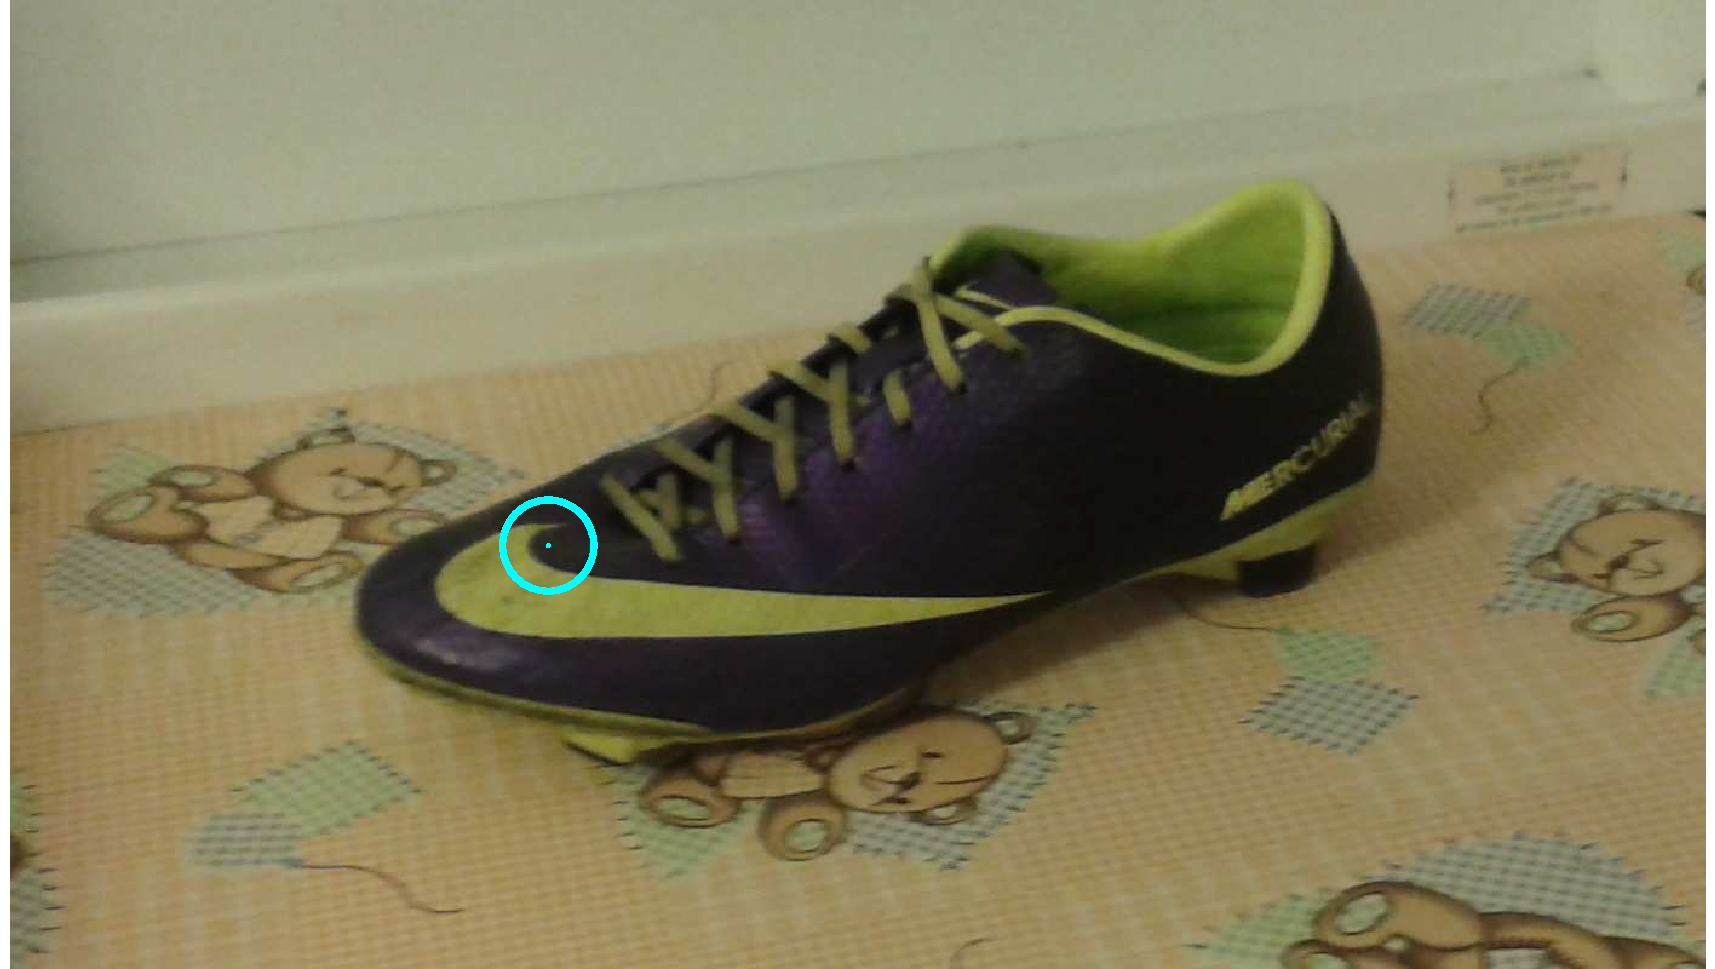
\includegraphics[width=\textwidth, clip=true, trim=165 50 155 68]{img/shoeDescriptor.pdf}
	\end{subfigure}
	\begin{subfigure}[t]{0.40\textwidth}
		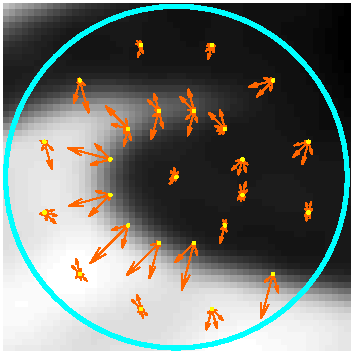
\includegraphics[width=\textwidth, clip=true, trim=1 1 1 1]{img/shoeDescriptorZoom.pdf}
	\end{subfigure}
\end{figure}
\end{frame}
%
\begin{frame}{Image transformations}
\begin{figure}
\centering
	\begin{subfigure}[t]{0.4\textwidth}
		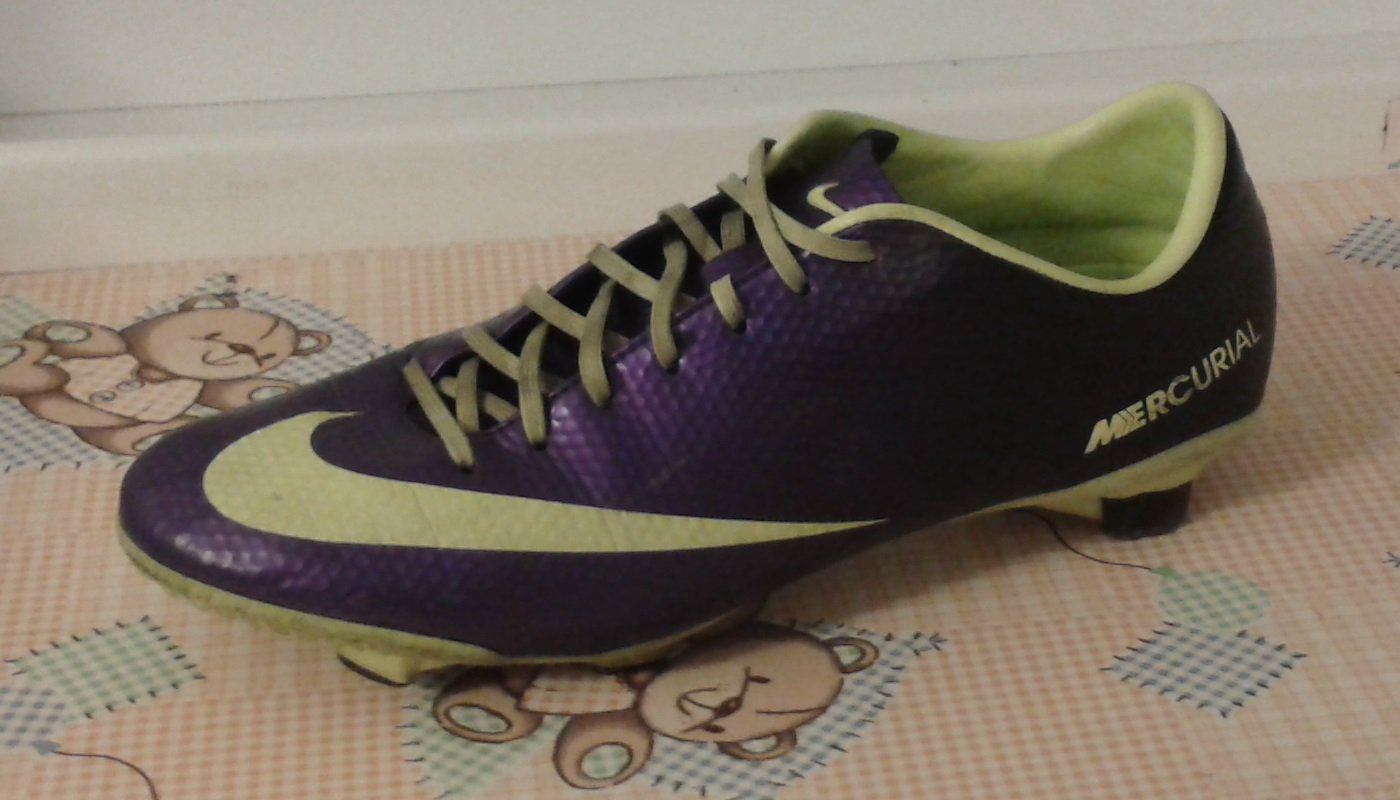
\includegraphics[width=\textwidth]{img/shoeOriginal.jpg}
	\end{subfigure}\\
	\vspace{0.75mm}
	\begin{subfigure}[t]{0.4\textwidth}
		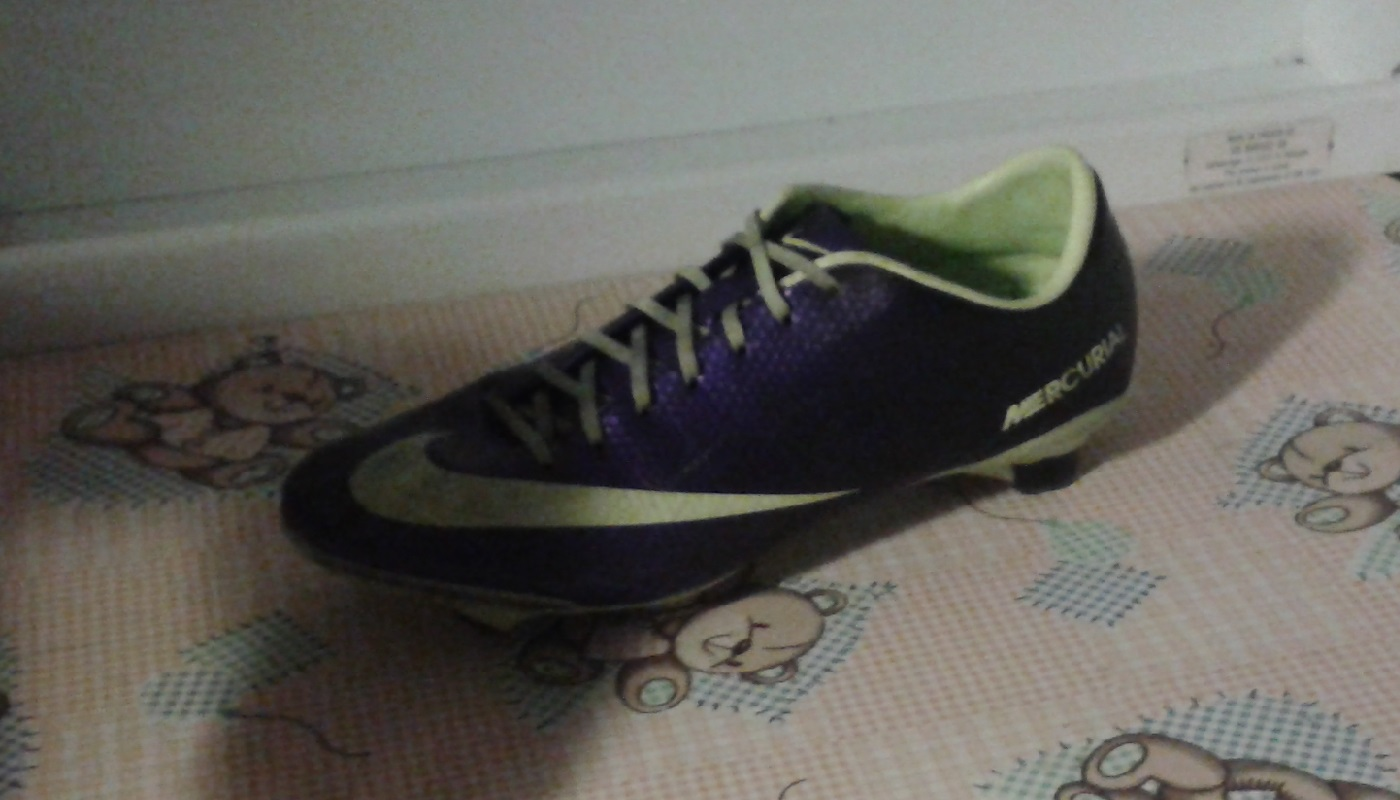
\includegraphics[width=\textwidth]{img/shoeShadow.jpg}
	\end{subfigure}
	\begin{subfigure}[t]{0.4\textwidth}
		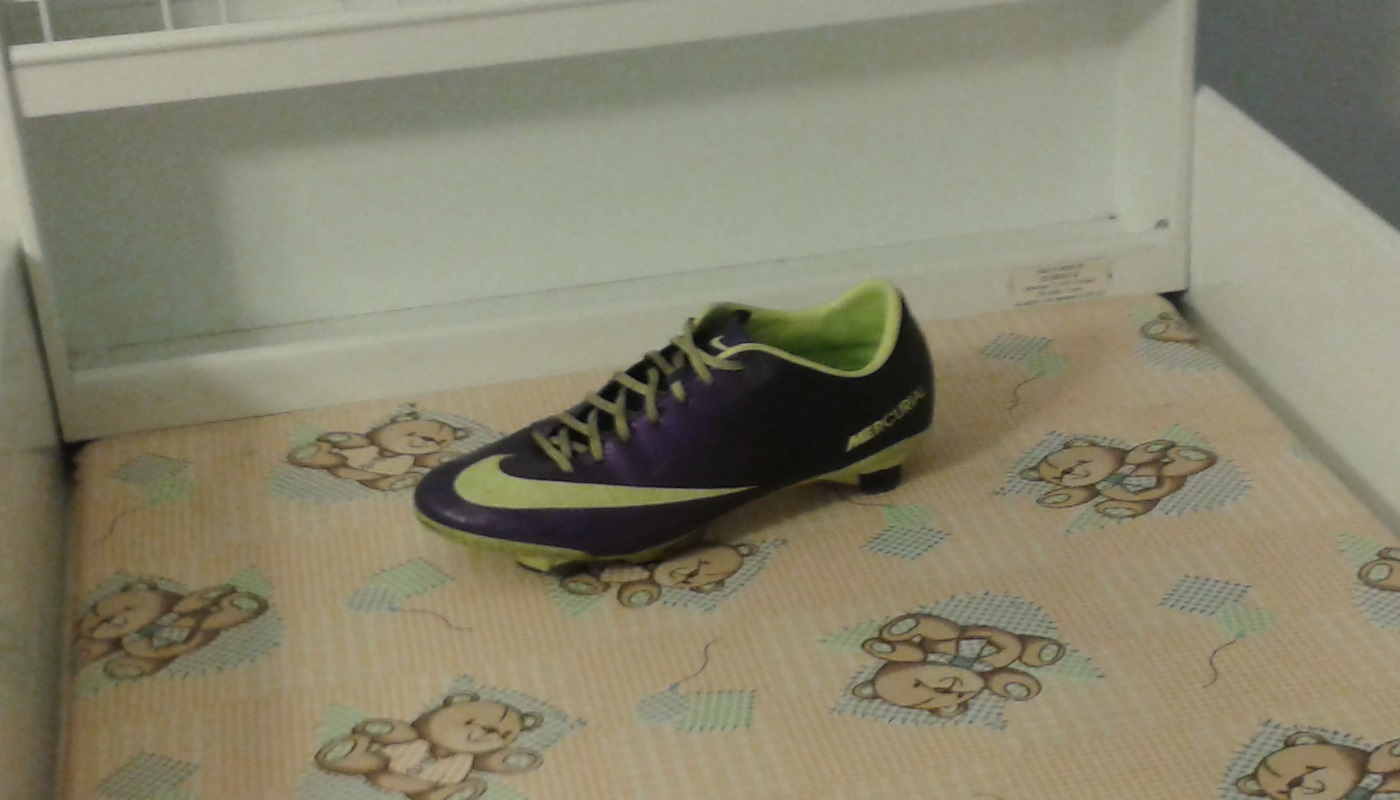
\includegraphics[width=\textwidth]{img/shoeScale.jpg}
	\end{subfigure}\\
	\vspace{0.75mm}
	\begin{subfigure}[t]{0.4\textwidth}
		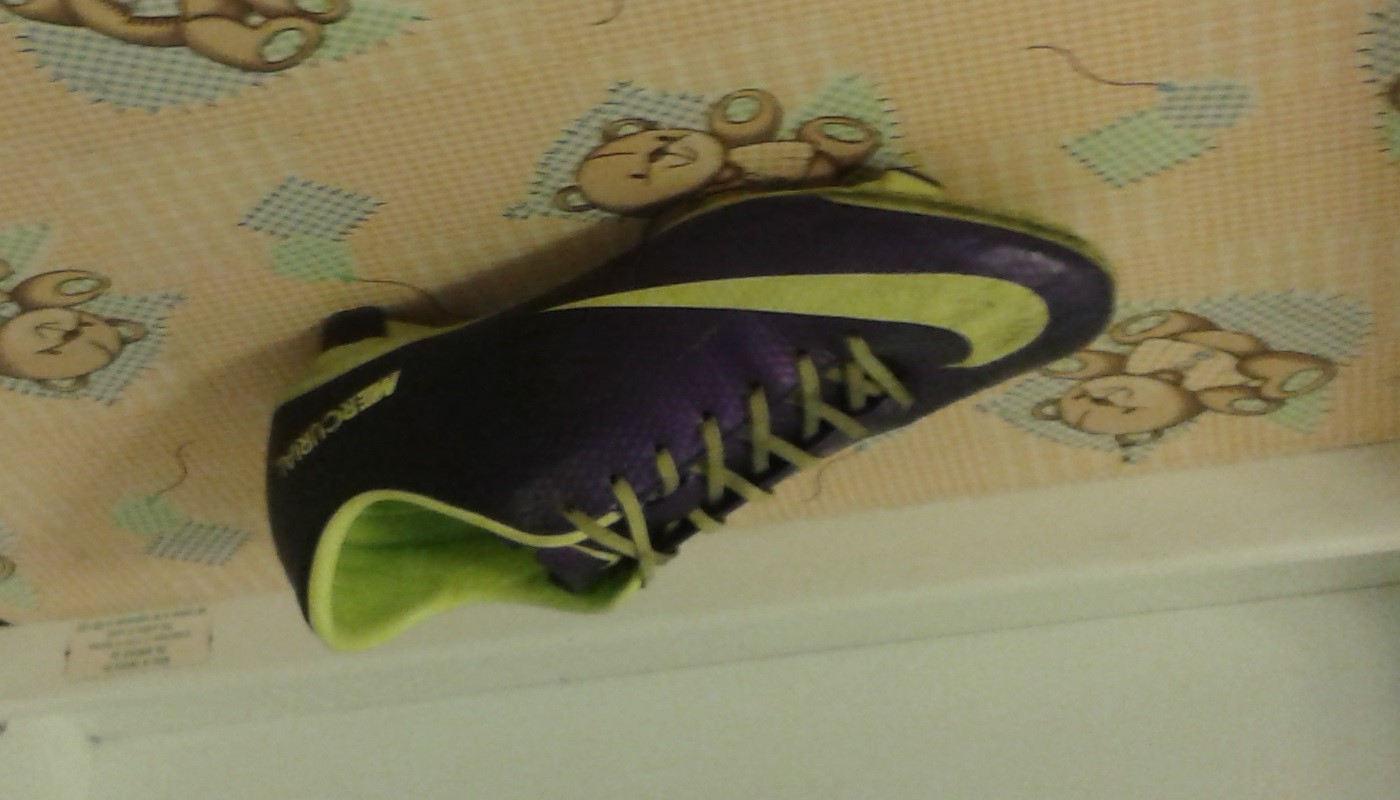
\includegraphics[width=\textwidth]{img/shoeRotation.jpg}
	\end{subfigure}
	\begin{subfigure}[t]{0.4\textwidth}
		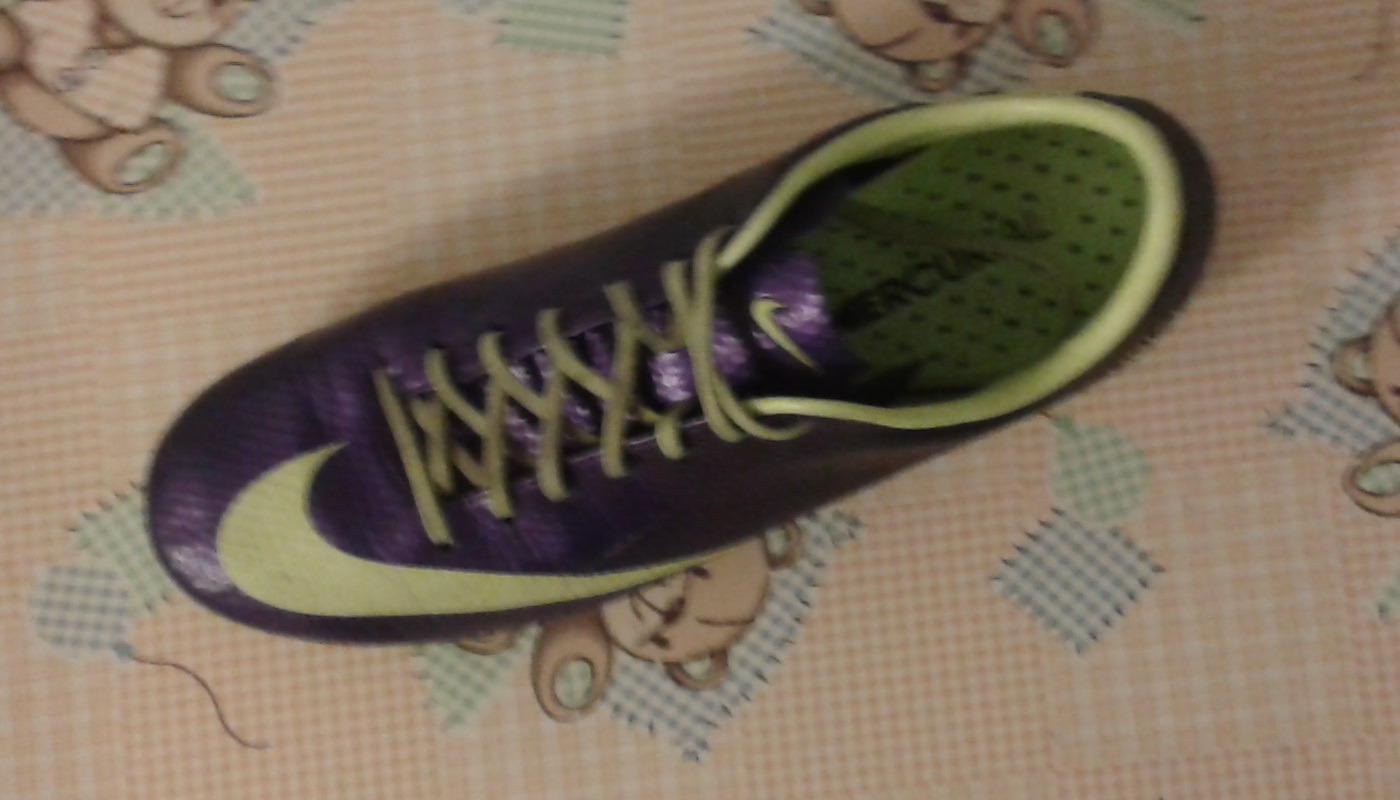
\includegraphics[width=\textwidth]{img/shoeAbove.jpg}
	\end{subfigure}
\end{figure}
\end{frame}
%
\begin{frame}{Scale-space}
\begin{figure}[p]
	\centering
	\begin{subfigure}[t]{0.4\textwidth}
		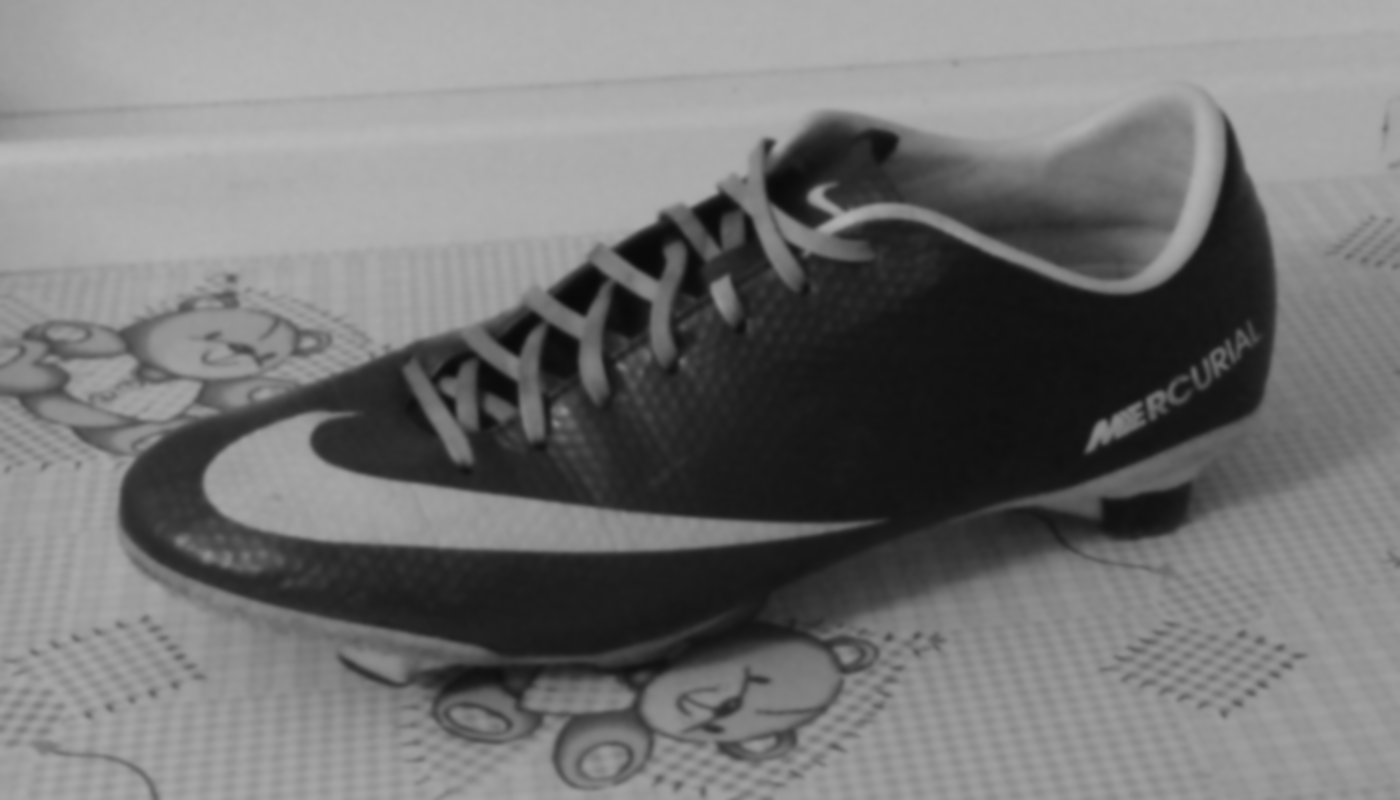
\includegraphics[width=\textwidth]{img/scaleSpaceTheory_2.png}
	\end{subfigure}
	\begin{subfigure}[t]{0.4\textwidth}
		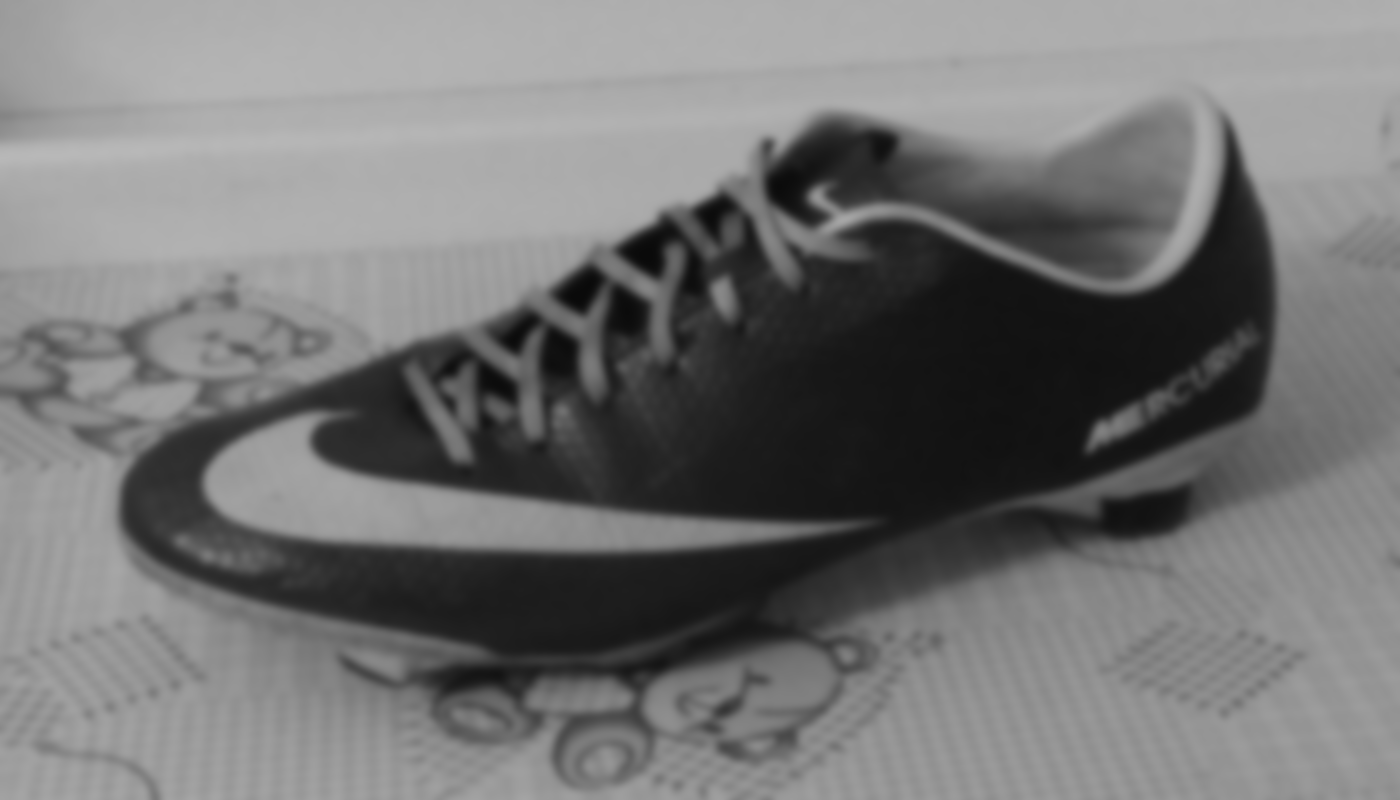
\includegraphics[width=\textwidth]{img/scaleSpaceTheory_4.png}
	\end{subfigure}\\
	\vspace{0.75mm}
	\begin{subfigure}[t]{0.4\textwidth}
		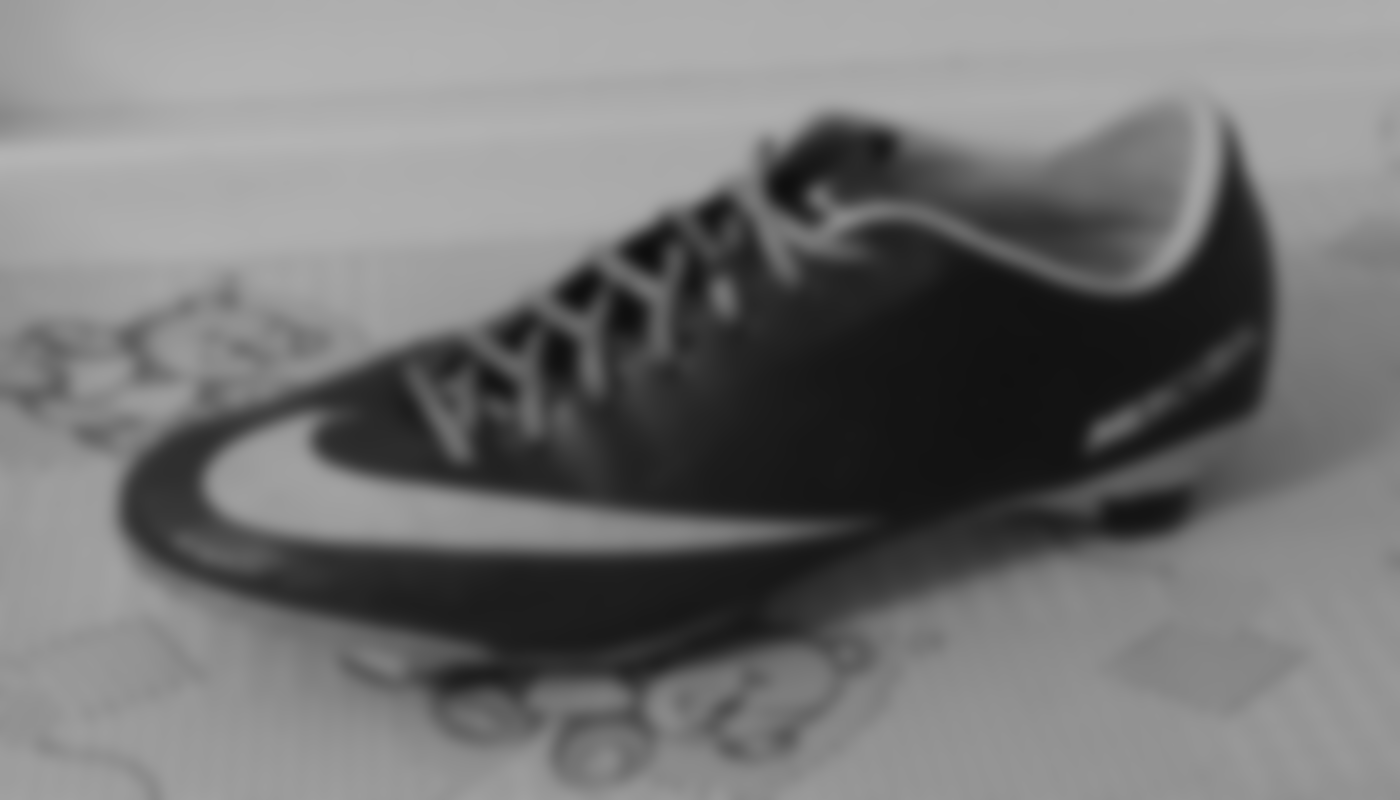
\includegraphics[width=\textwidth]{img/scaleSpaceTheory_8.png}
	\end{subfigure}
	\begin{subfigure}[t]{0.4\textwidth}
		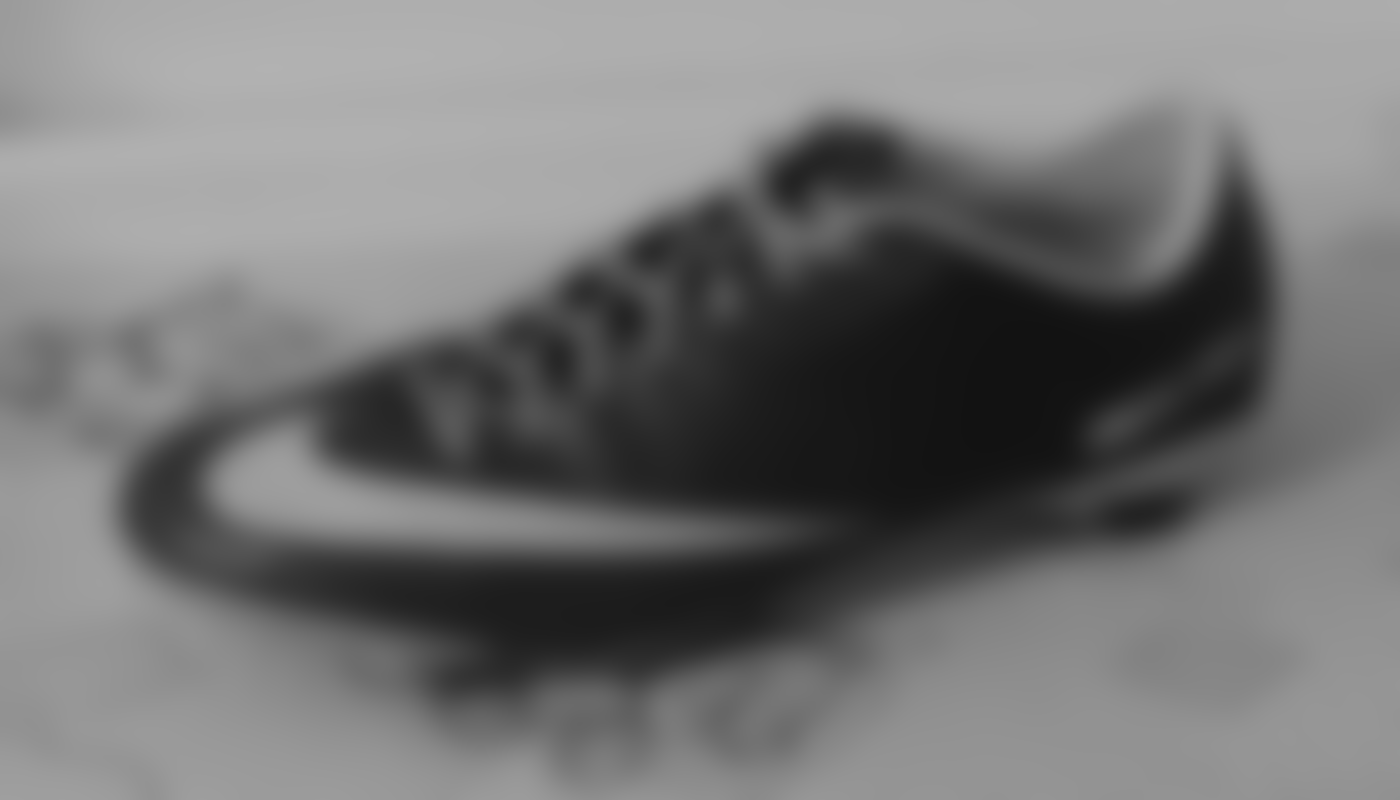
\includegraphics[width=\textwidth]{img/scaleSpaceTheory_16.png}
	\end{subfigure}\\
	\vspace{0.75mm}
	\begin{subfigure}[t]{0.4\textwidth}
		
\includegraphics[width=\textwidth]{img/scaleSpaceTheory_32.png}
	\end{subfigure}
	\begin{subfigure}[t]{0.4\textwidth}
		
\includegraphics[width=\textwidth]{img/scaleSpaceTheory_64.png}
	\end{subfigure}
\end{figure}
\end{frame}
%
\begin{frame}[c]{Applications}
\begin{figure}
\centering
	\begin{subfigure}[t]{0.49\textwidth}
		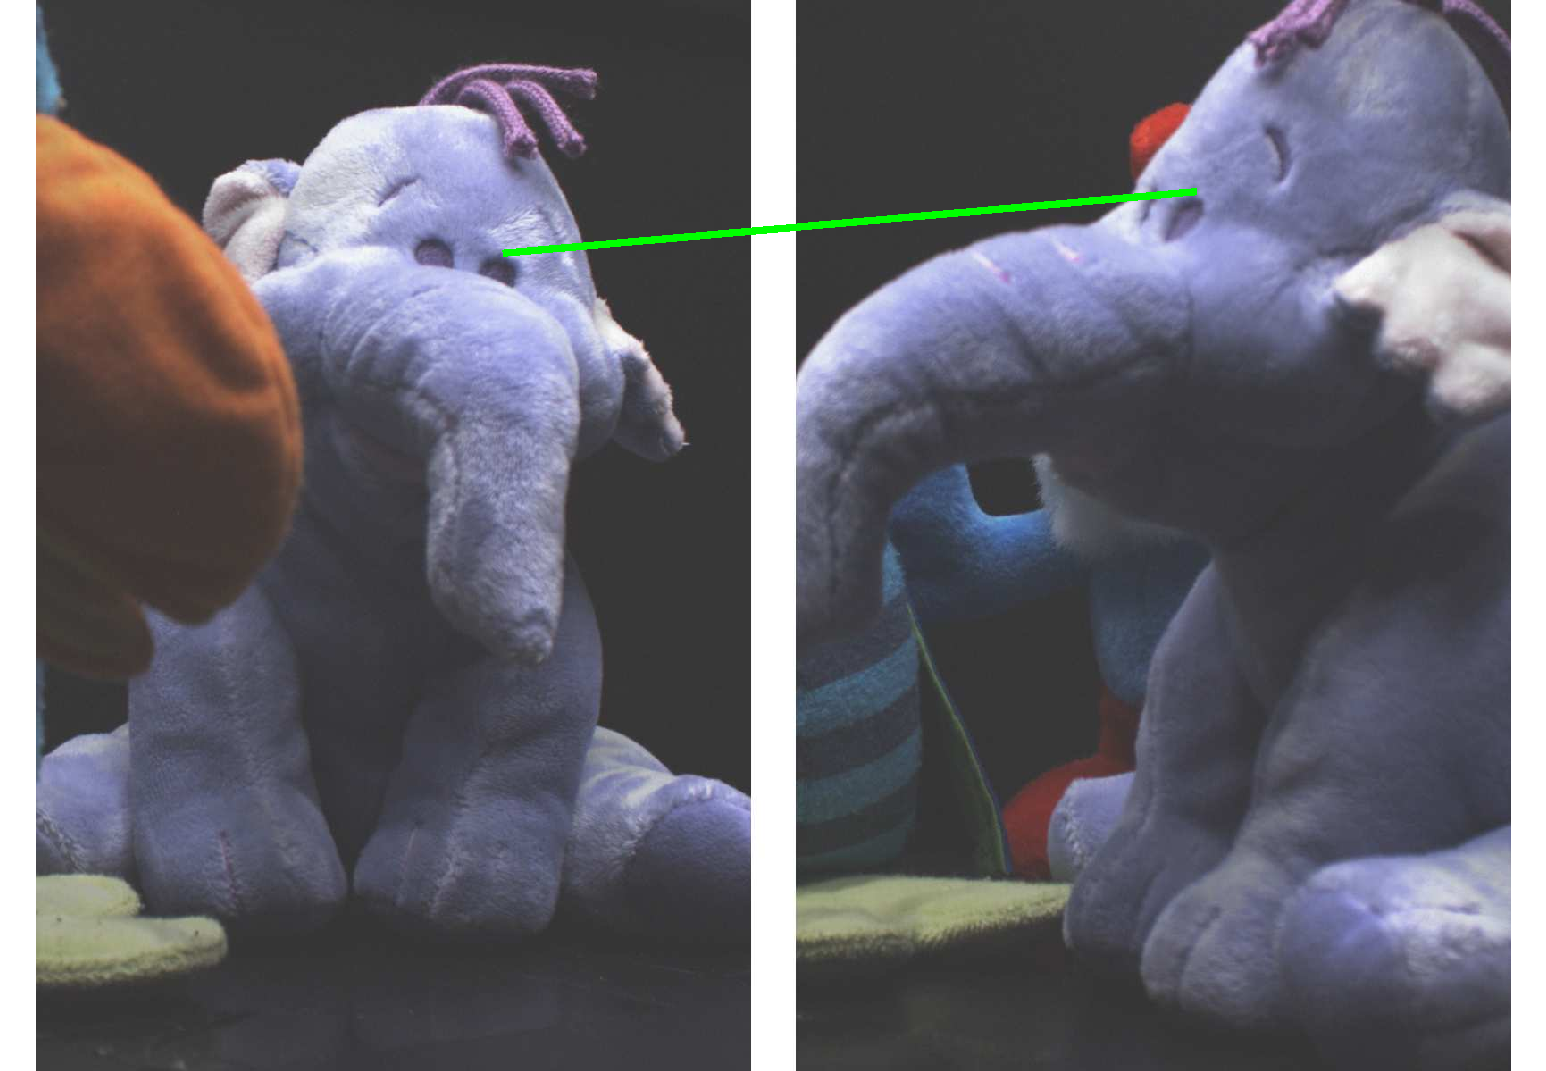
\includegraphics[width=\textwidth]{img/introductionIC.pdf}
		\caption{Image correspondence}
	\end{subfigure}
	\begin{subfigure}[t]{0.49\textwidth}
		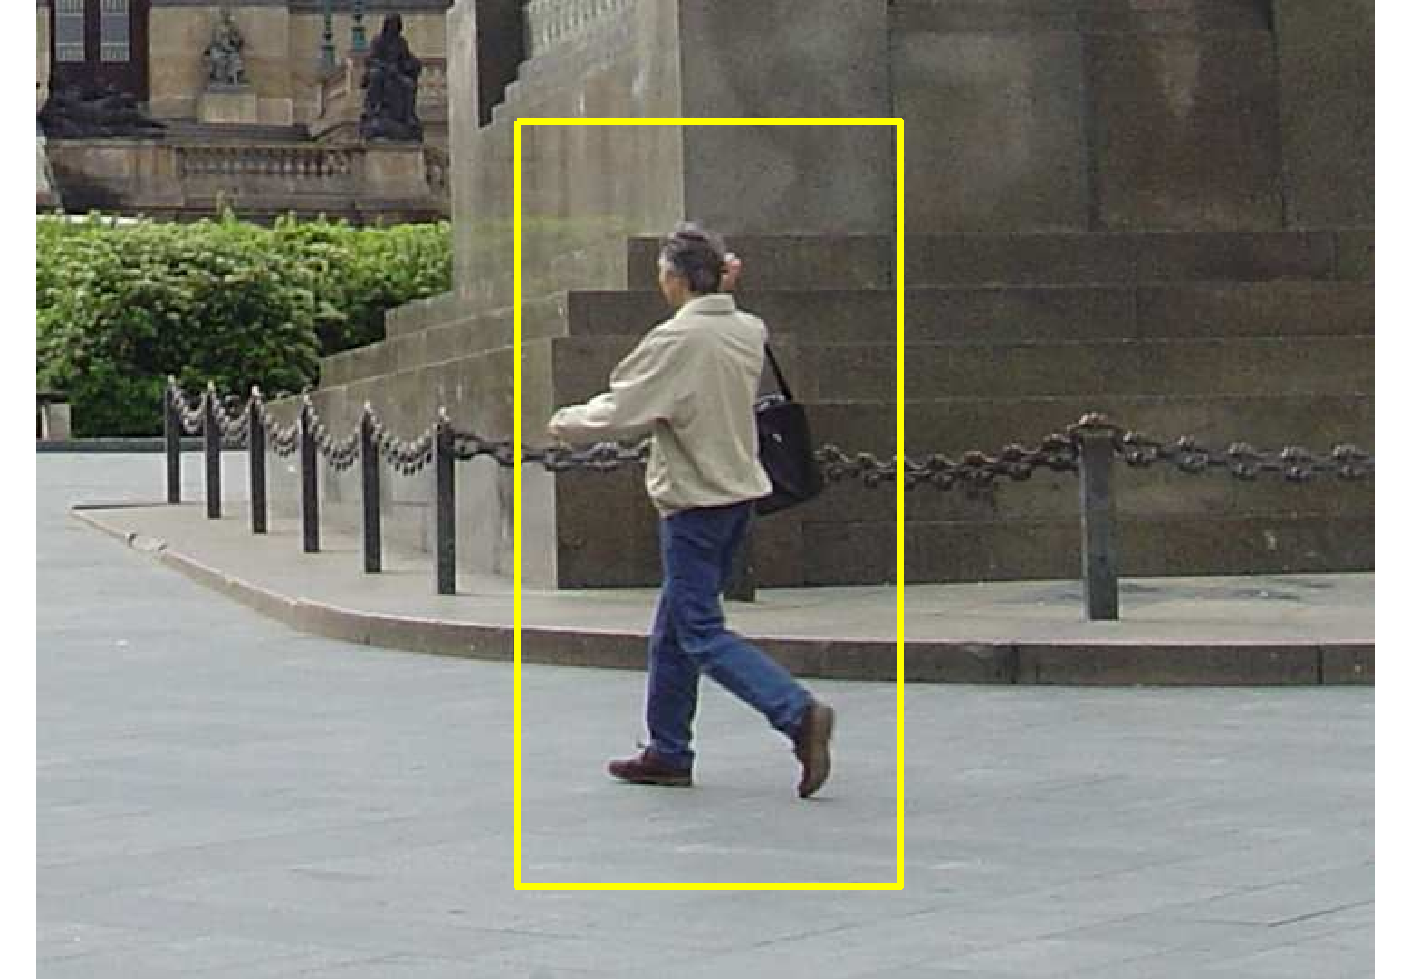
\includegraphics[width=\textwidth]{img/introductionOD.pdf}
		\caption{Pedestrian detection}
	\end{subfigure}
\end{figure}
\end{frame}
%
\section{Image correspondence}
%
\begin{frame}{Interest point detection}
\begin{figure}
\centering
	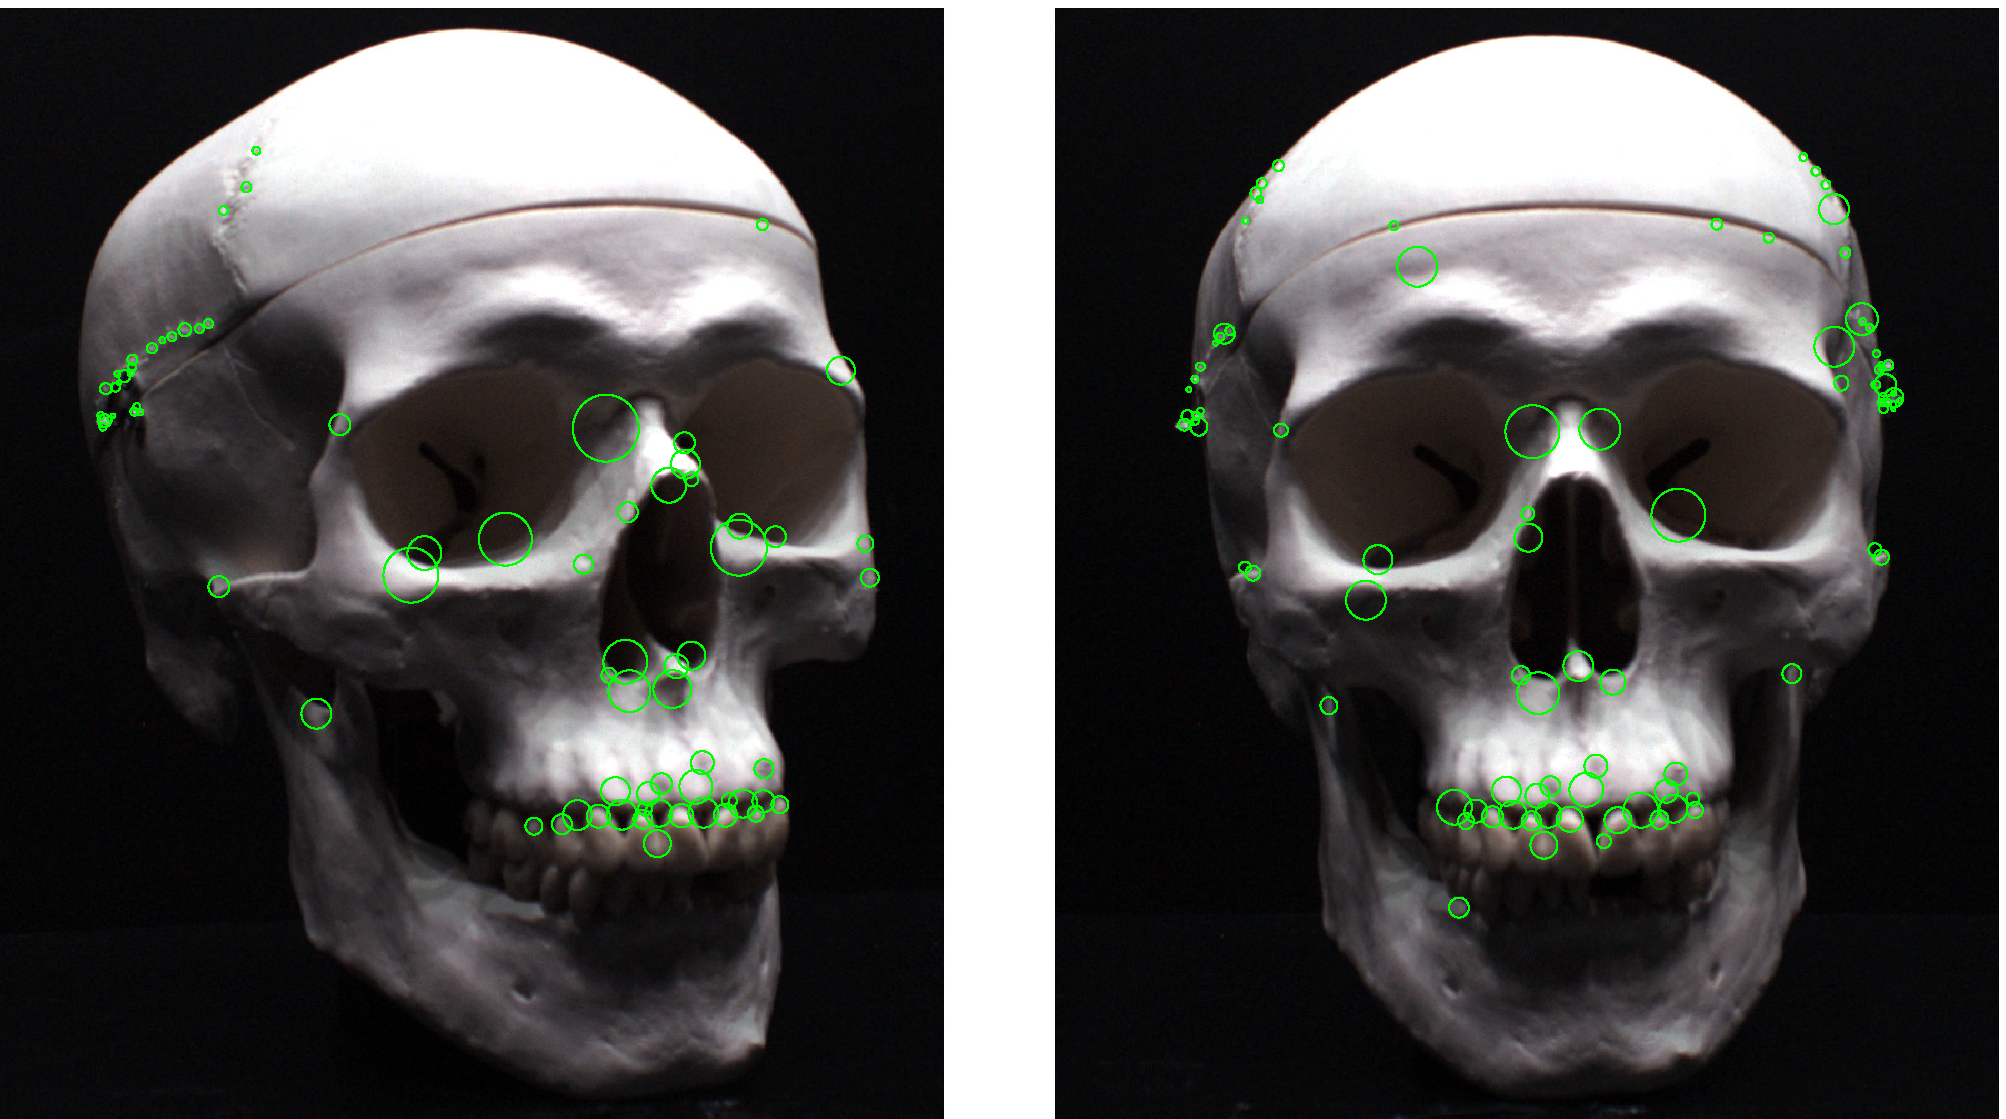
\includegraphics[width=\textwidth]{img/imageCorrespondenceInterestPoints.pdf}
\end{figure}
\end{frame}
%
\begin{frame}{Matching strategy}
\begin{figure}
\centering
	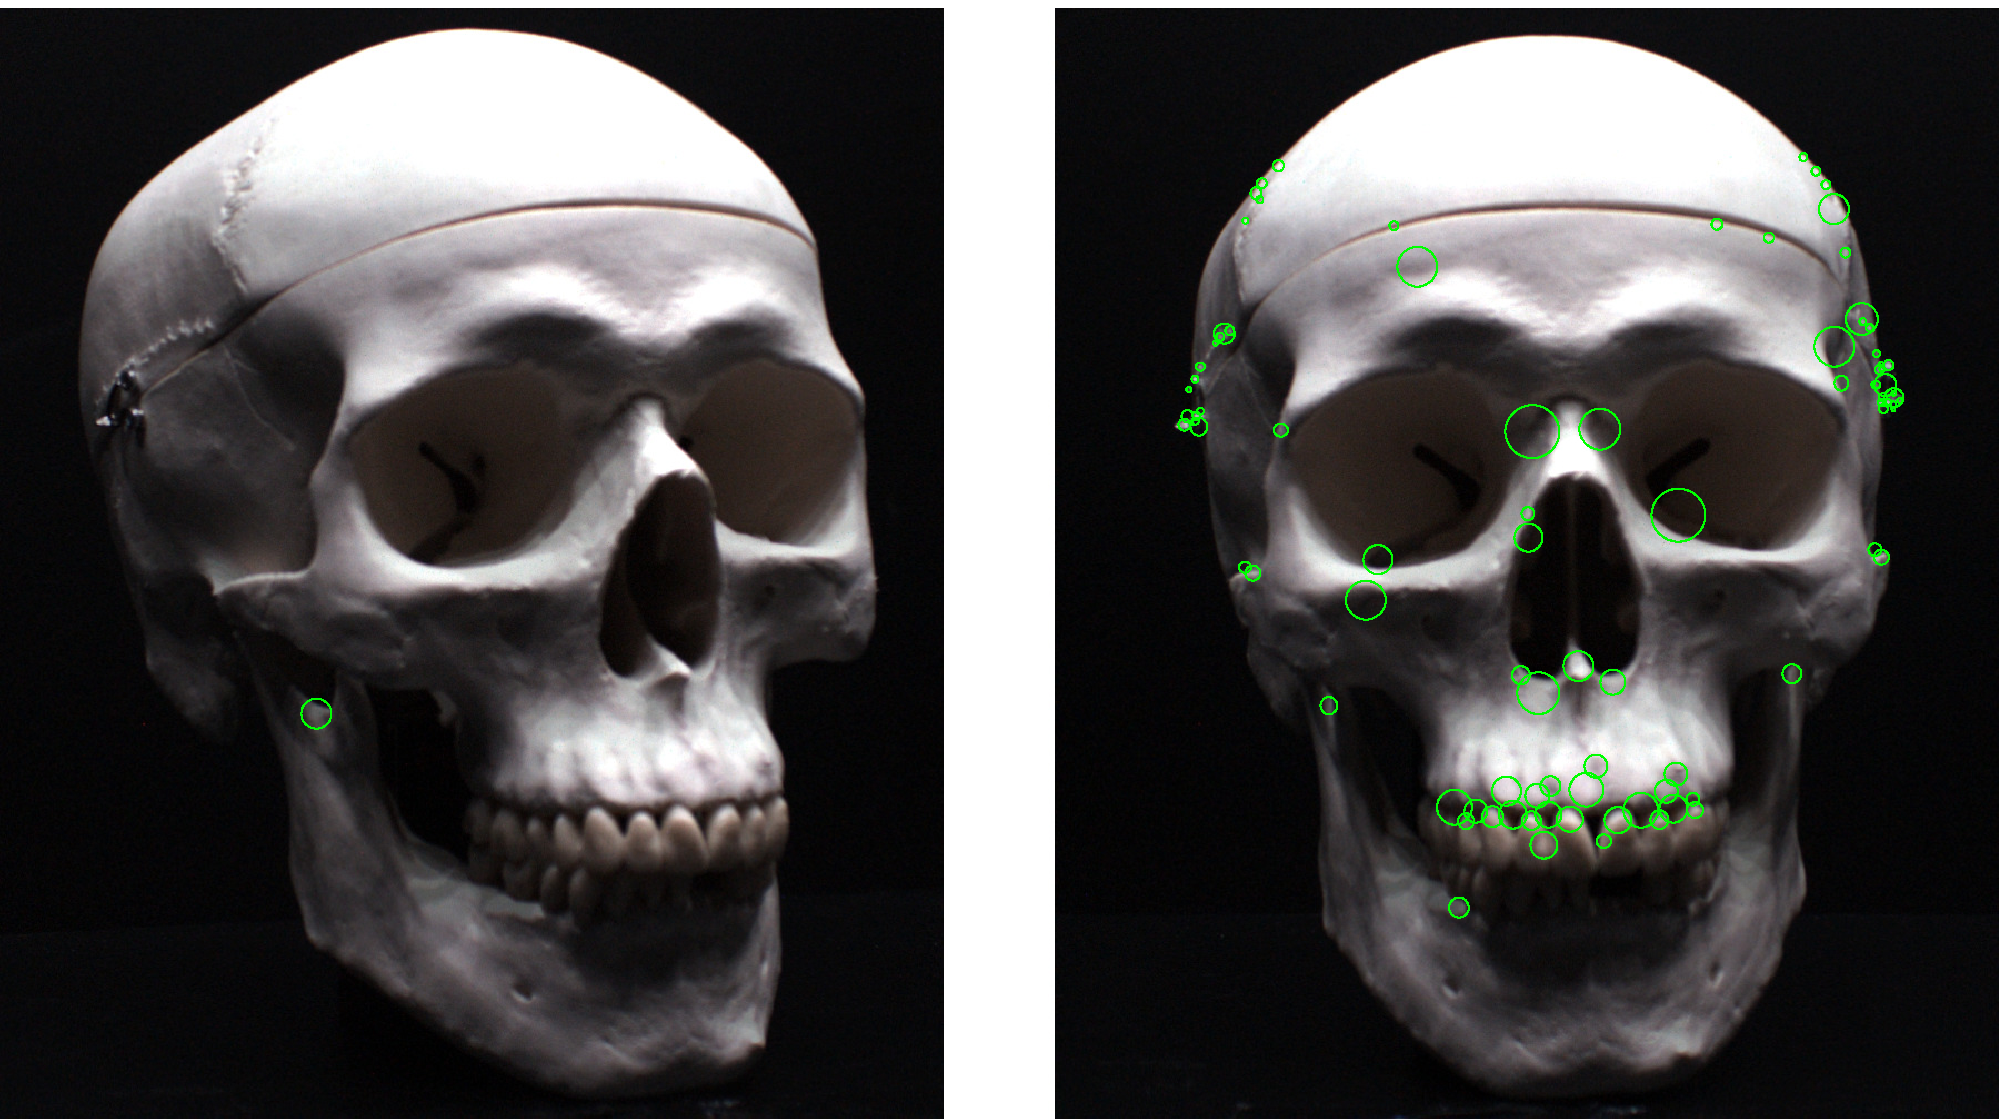
\includegraphics[width=\textwidth]{img/imageCorrespondenceExample1.pdf}
\end{figure}
\end{frame}
\begin{frame}{Matching strategy}
\begin{figure}
\centering
	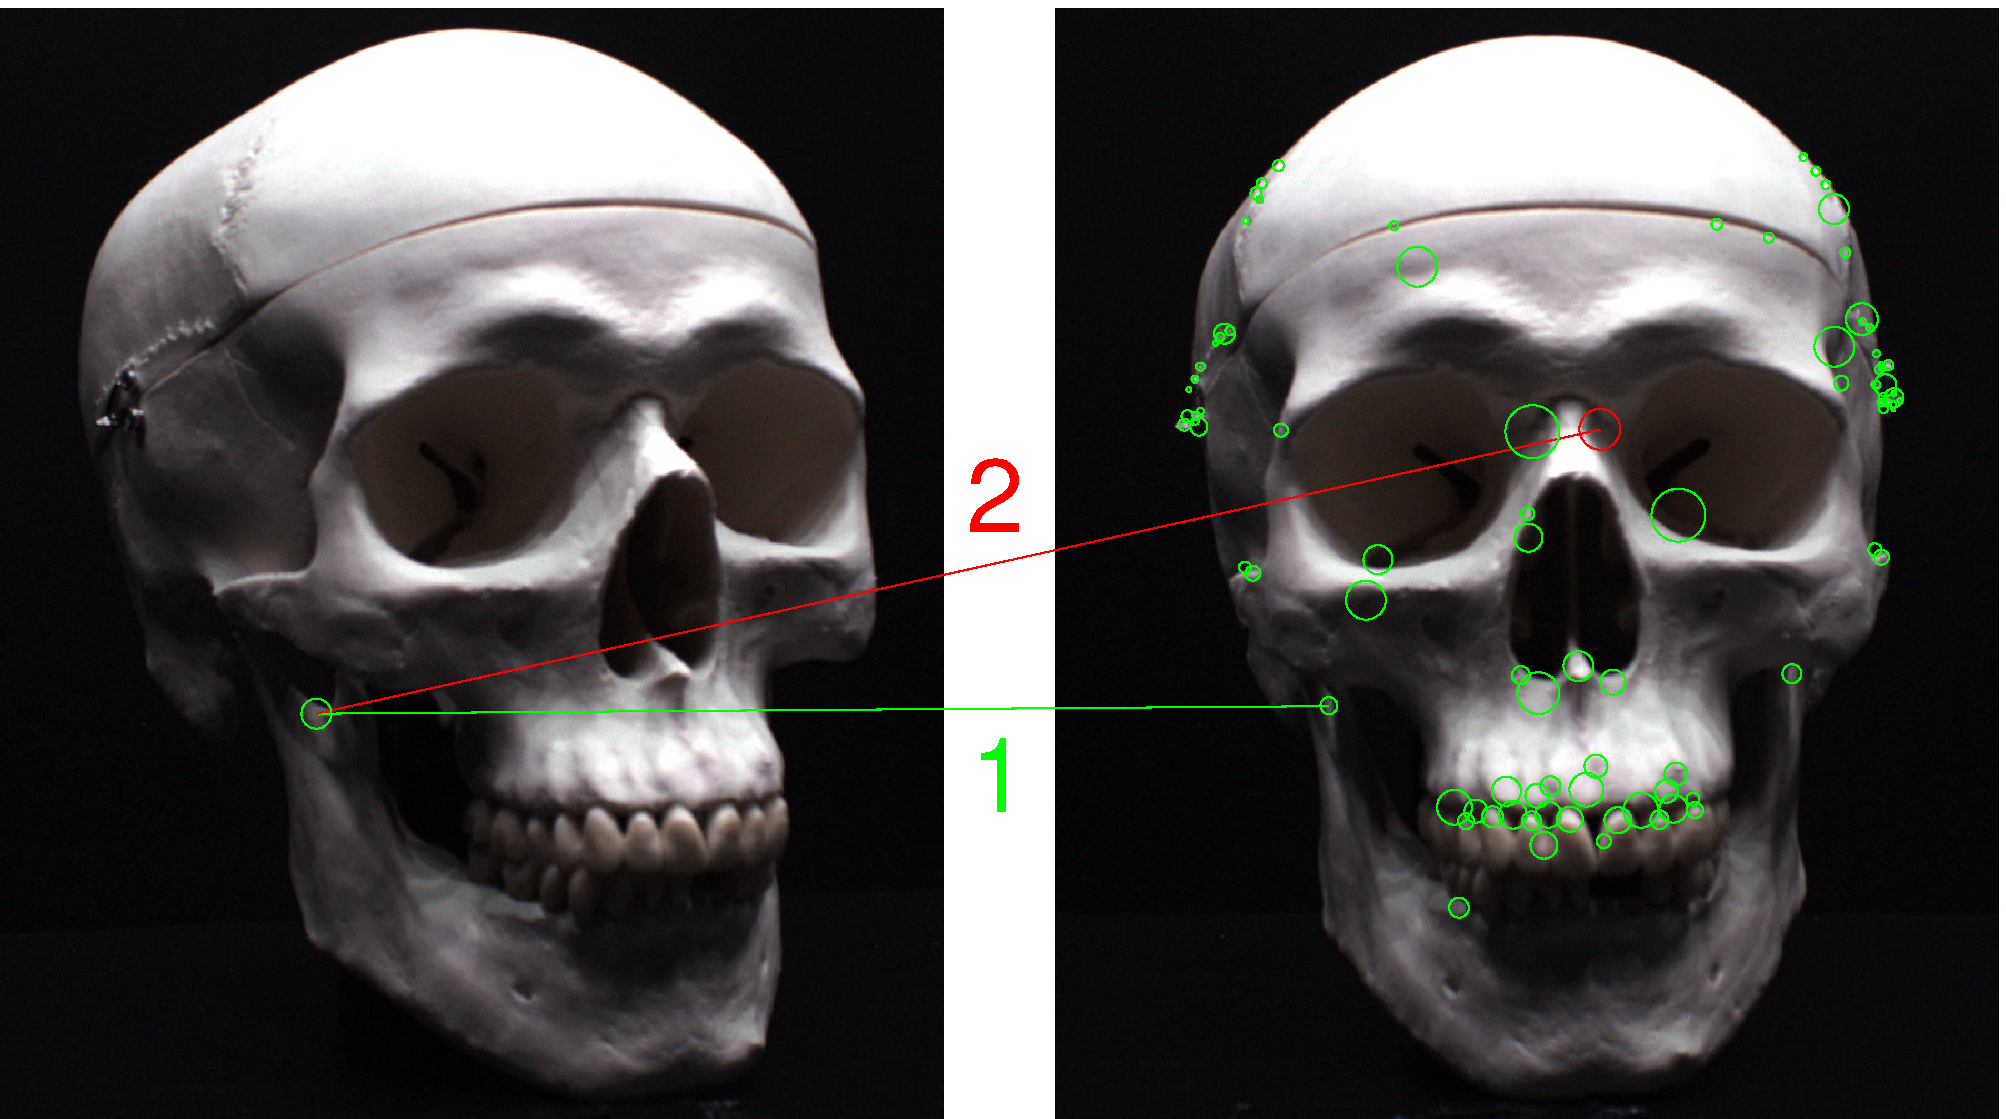
\includegraphics[width=\textwidth]{img/imageCorrespondenceExample2.pdf}
\end{figure}
\end{frame}
\begin{frame}{Matching strategy}
\begin{figure}
\centering
	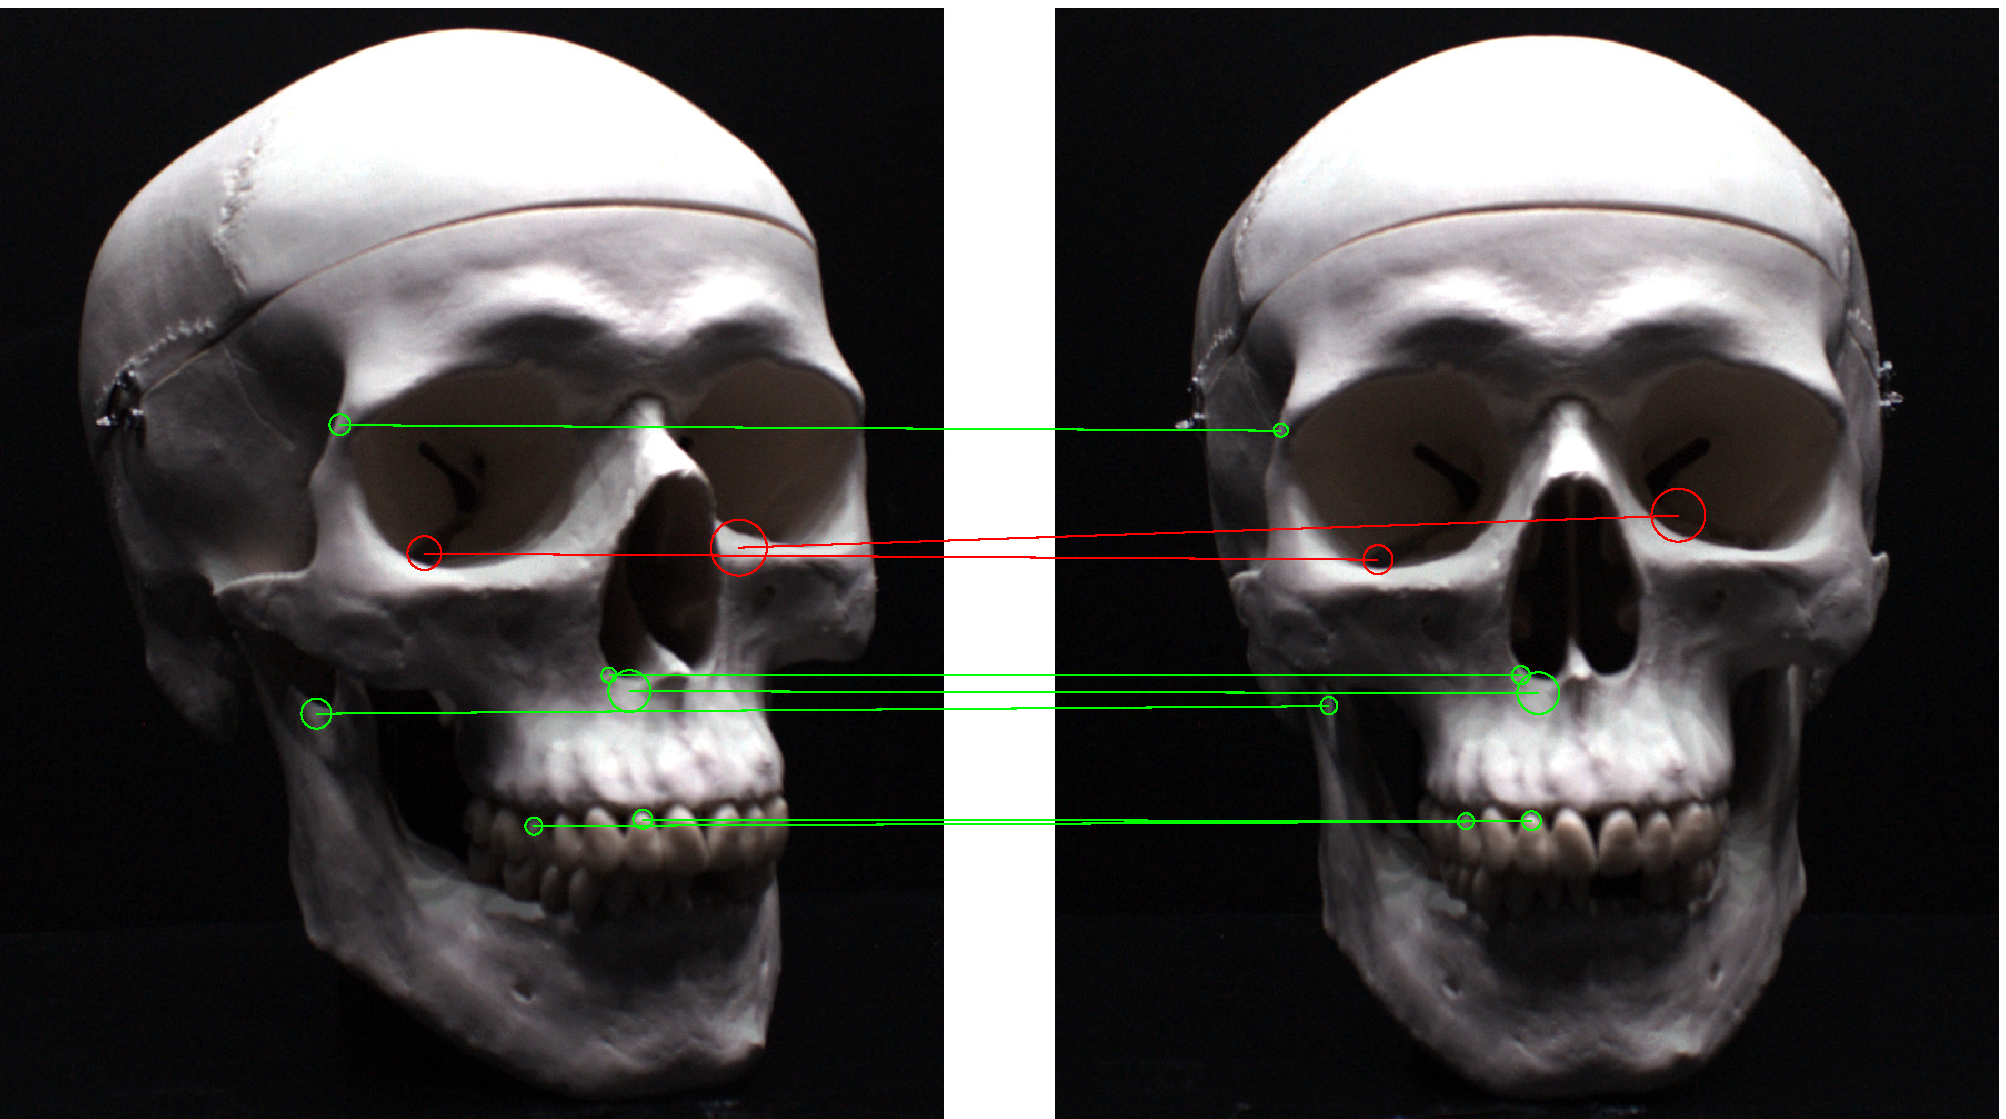
\includegraphics[width=\textwidth]{img/imageCorrespondenceExample3.pdf}
\end{figure}
\end{frame}
%
\begin{frame}{Proposed descriptor}
\begin{align*}
H_j(f_i) = \int F(\x) A_j (\x) P (\x) B(\x; f_i,f) \,\text{d} \x
\end{align*}
\begin{minipage}[t]{0.58\textwidth}
	where
	\begin{itemize}
	\item[] $i$ is the bin number
	\item[] $j$ is the cell number
	\end{itemize}
\end{minipage}
\begin{minipage}[t]{0.4\textwidth}
	\begin{figure}
		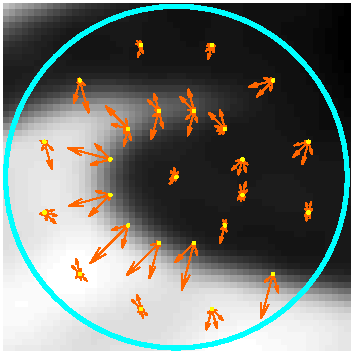
\includegraphics[width=\textwidth, clip=true, trim=1 1 1 1]{img/shoeDescriptorZoom.pdf}
	\end{figure}
\end{minipage}
\end{frame}
%
\begin{frame}{Histogram domain}
\begin{align*}
\textcolor{faded}{H_j(f_i) = \int \textcolor{black}{F(\x)} A_j (\x) P (\x) B(\x; f_i,\textcolor{black}{f}) \,\text{d} \x}
\end{align*}
Bin value function $f$

Magnitude function $F$
\end{frame}
%
\begin{frame}{Gradient orientation}
\begin{figure}
\centering
	\begin{subfigure}[t]{0.75\textwidth}
		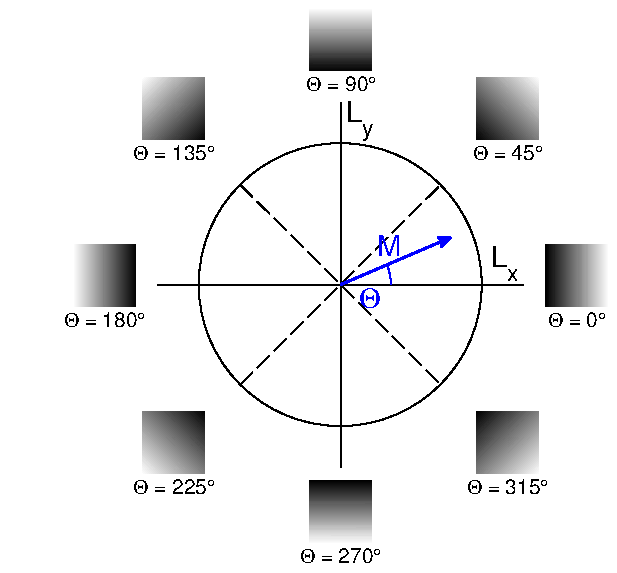
\includegraphics[width=\textwidth]{../report/img/gradientOrientationTheory.pdf}
	\end{subfigure}
\end{figure}
\end{frame}
%
\begin{frame}{Shape index}
\begin{figure}
\centering
	\begin{subfigure}[t]{0.75\textwidth}
		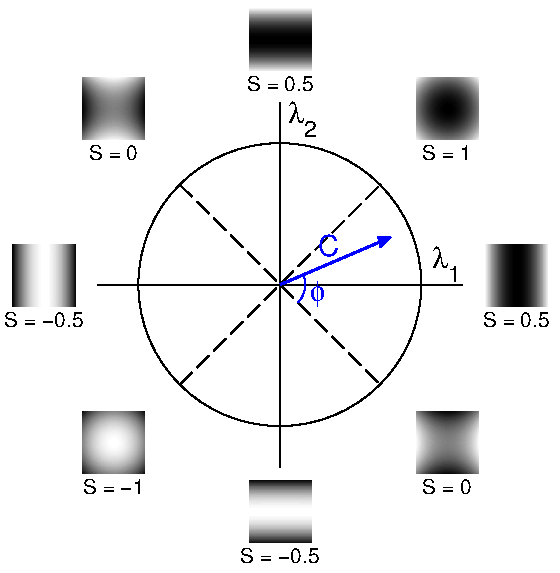
\includegraphics[width=\textwidth]{../report/img/shapeIndexTheory.pdf}
	\end{subfigure}
\end{figure}
\end{frame}
%
\begin{frame}{Local magnitude normalization}
\begin{figure}[p]
	\centering
	\begin{subfigure}[t]{0.4\textwidth}
		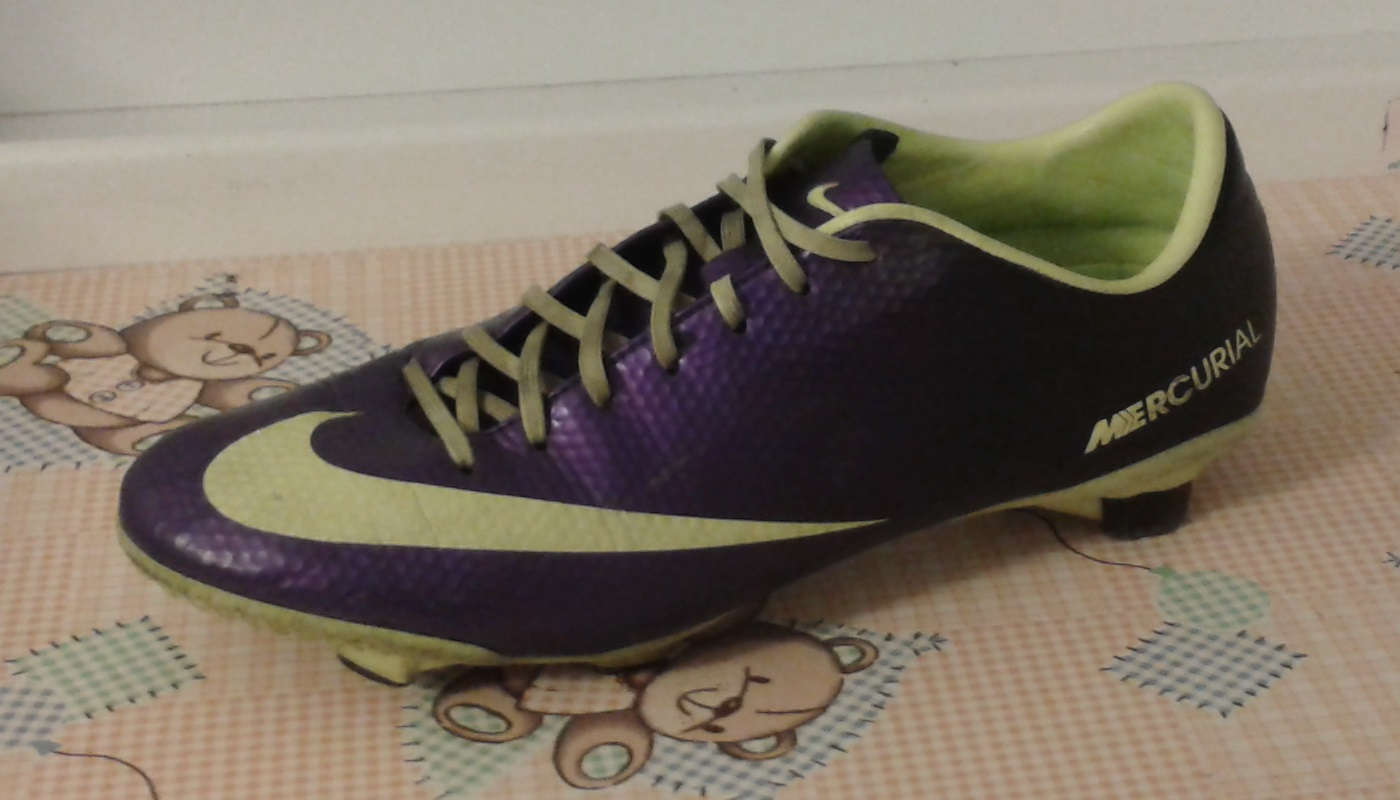
\includegraphics[width=\textwidth]{img/pixelNormalizationExample1.png}
	\end{subfigure}
	\hspace{0.5cm}
	\begin{subfigure}[t]{0.4\textwidth}
		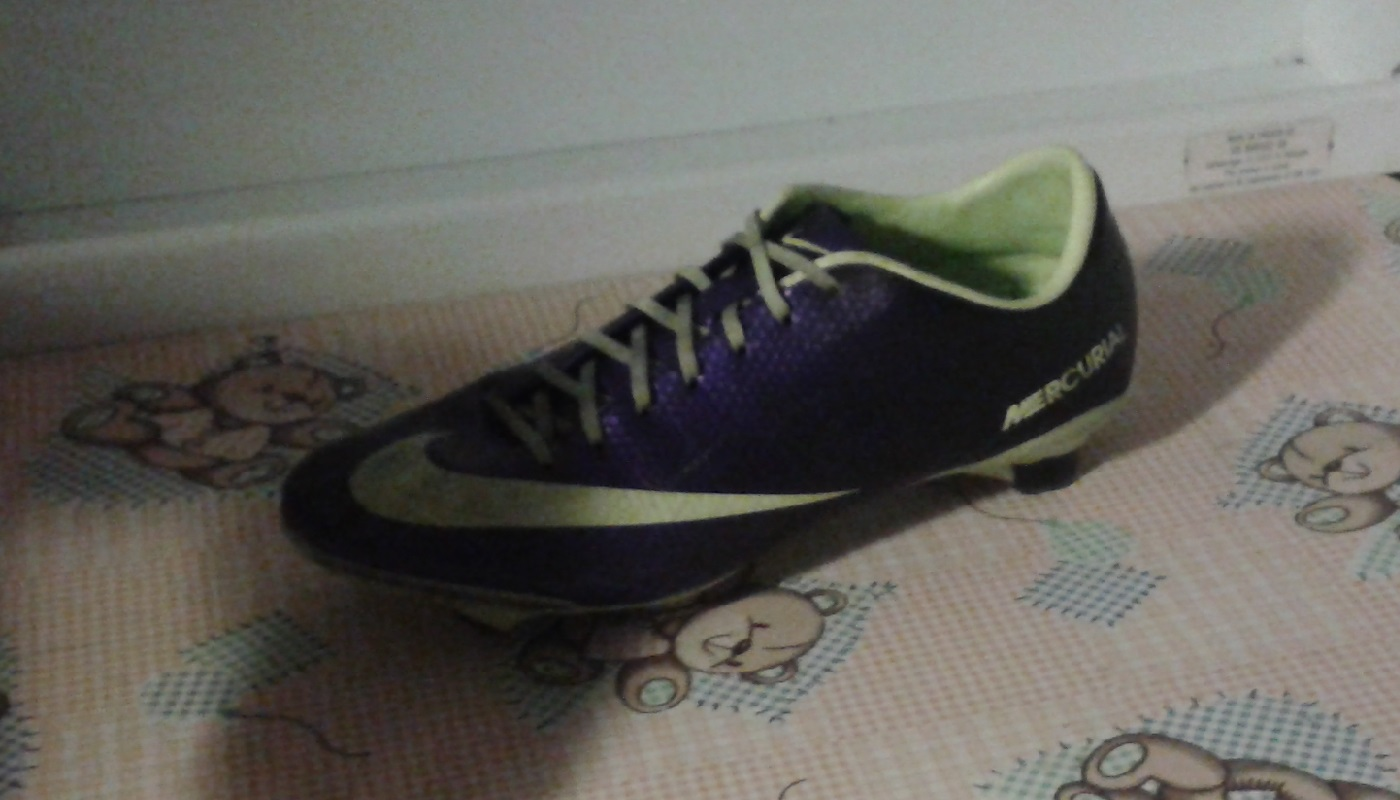
\includegraphics[width=\textwidth]{img/pixelNormalizationExample2.png}
	\end{subfigure}\\
	\vspace{0.75mm}
	\begin{subfigure}[t]{0.4\textwidth}
		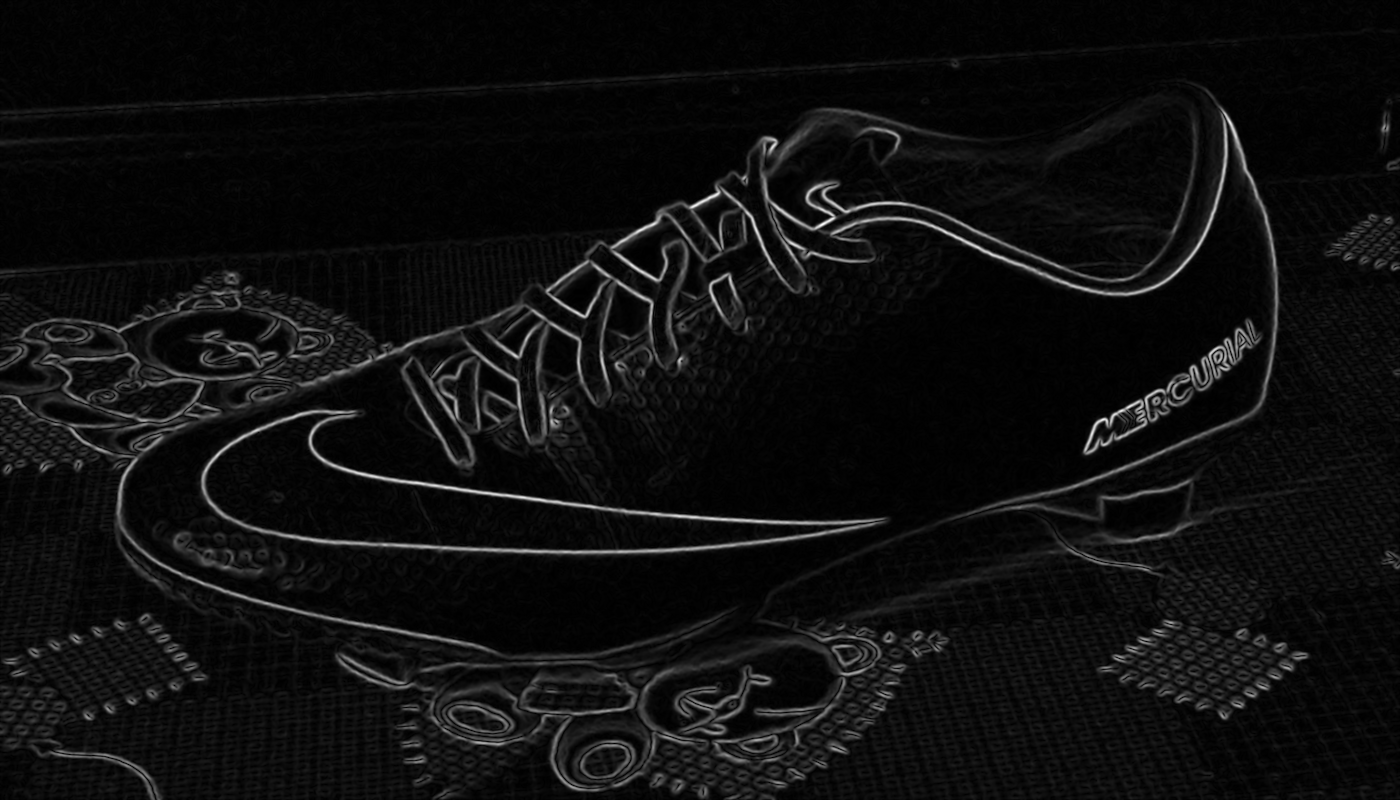
\includegraphics[width=\textwidth]{img/pixelNormalizationExample3.png}
	\end{subfigure}
	\hspace{0.5cm}
	\begin{subfigure}[t]{0.4\textwidth}
		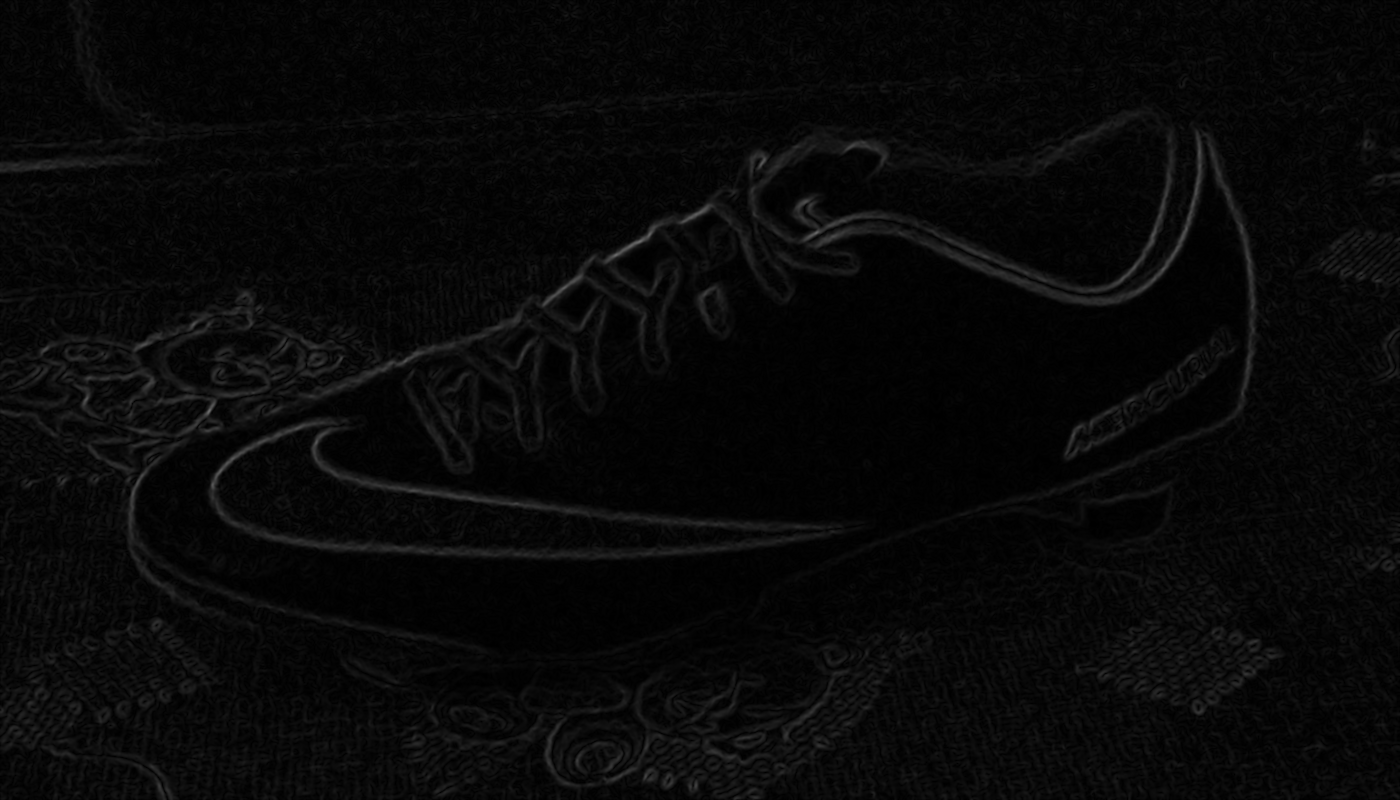
\includegraphics[width=\textwidth]{img/pixelNormalizationExample4.png}
	\end{subfigure}\\
	\vspace{0.75mm}
	\begin{subfigure}[t]{0.4\textwidth}
		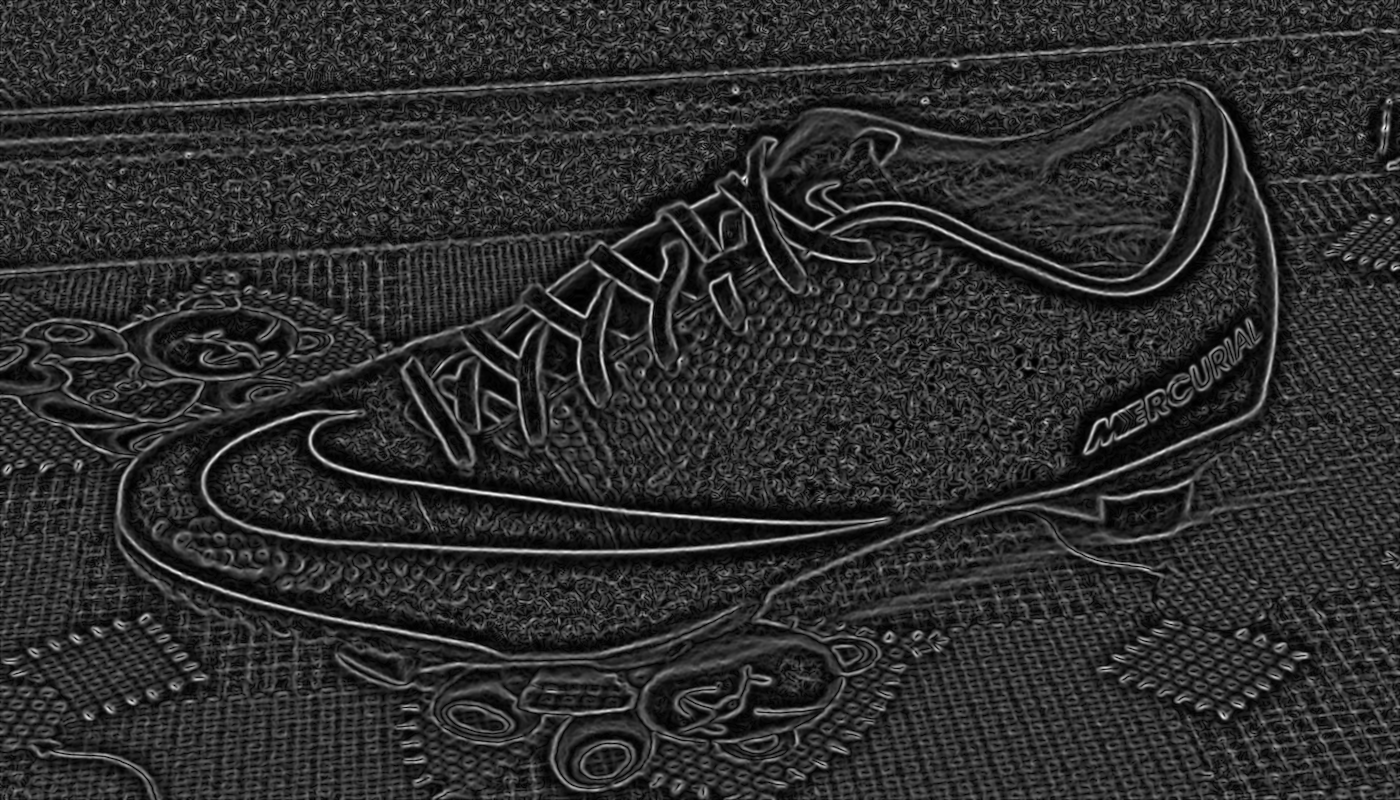
\includegraphics[width=\textwidth]{img/pixelNormalizationExample5.png}
	\end{subfigure}
	\hspace{0.5cm}
	\begin{subfigure}[t]{0.4\textwidth}
		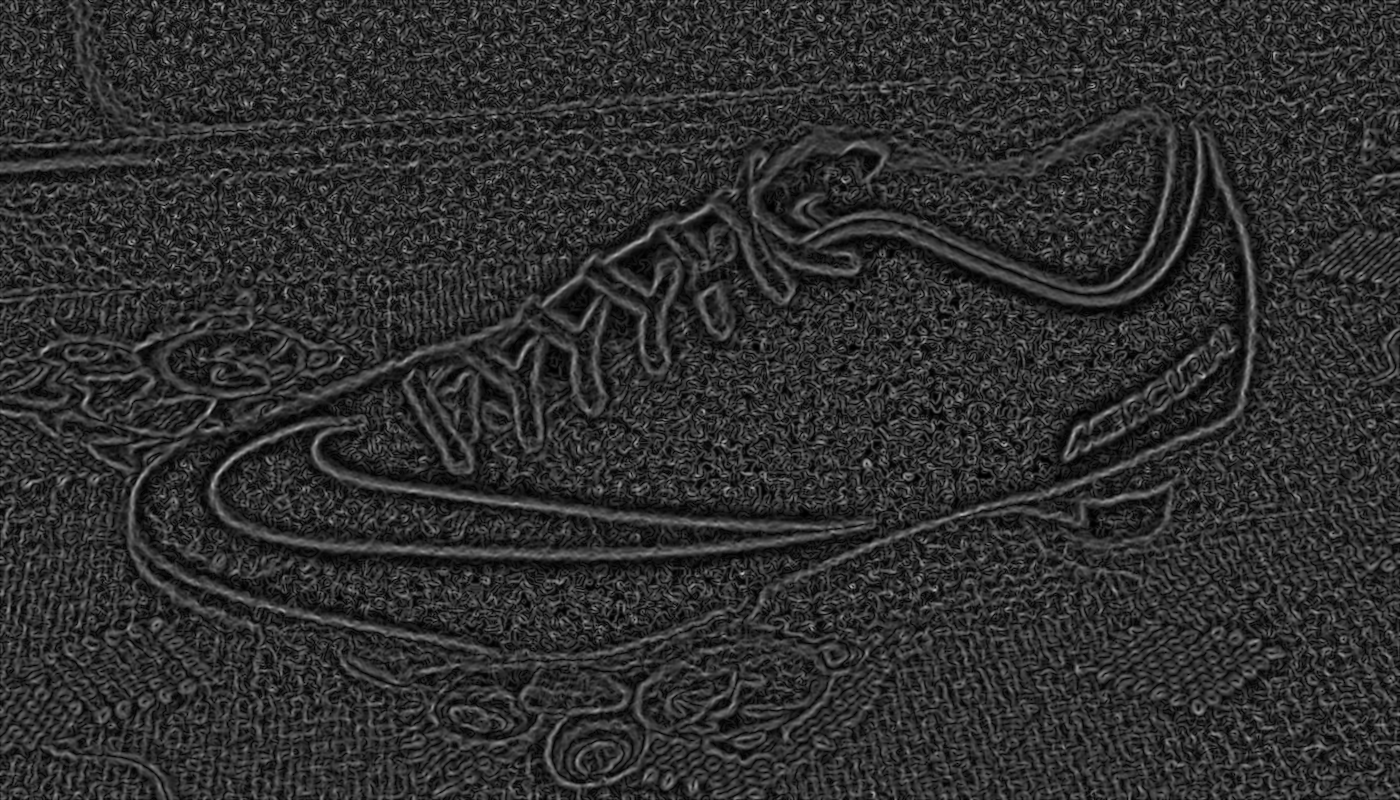
\includegraphics[width=\textwidth]{img/pixelNormalizationExample6.png}
	\end{subfigure}
\end{figure}
\end{frame}
%
\begin{frame}{Spatial weights}
\begin{align*}
\textcolor{faded}{H_j(f_i) = \int F(\x) \textcolor{black}{A_j (\x) P (\x)} B(\x; f_i,f) \,\text{d} \x}
\end{align*}
Cell aperture function $A_j$

Center aperture function $P$
\end{frame}
%
\begin{frame}{Cell aperture function}
\begin{figure}
\centering
	\begin{subfigure}[t]{\textwidth}
		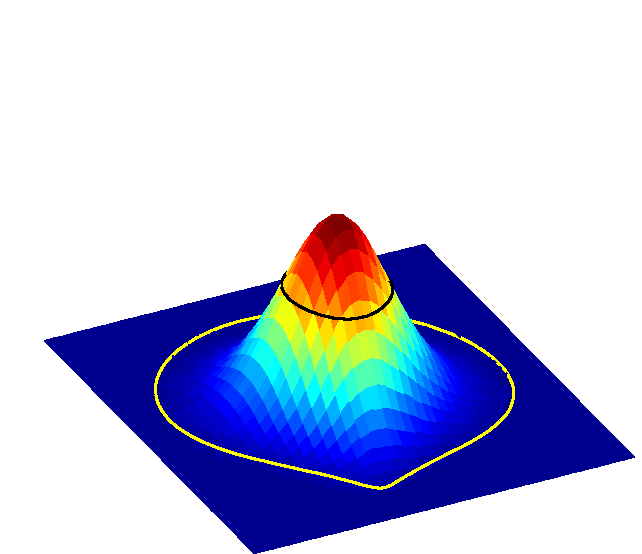
\includegraphics[width=\textwidth, clip=true, trim=0 0 0 90]{../defence/img/cellWindowPolar.pdf}
	\end{subfigure}
\end{figure}
\end{frame}
%
\begin{frame}{Grid of cells}
\begin{figure}
\centering
	\begin{subfigure}[t]{0.7\textwidth}
		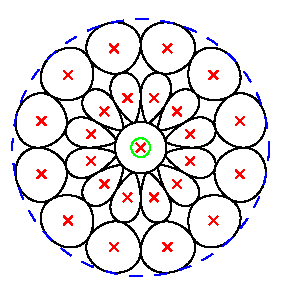
\includegraphics[width=\textwidth]{img/gridExample.pdf}
	\end{subfigure}
\end{figure}
\end{frame}
%
\begin{frame}{Bin weights}
\begin{align*}
\textcolor{faded}{H_j(f_i) = \int F(\x) A_j (\x) P (\x) \textcolor{black}{B(\x; f_i,f)} \,\text{d} \x}
\end{align*}
Bin aperture function $B$
\end{frame}
%
\begin{frame}{Bin weights}
\begin{figure}
\centering
	\begin{subfigure}[t]{1\textwidth}
		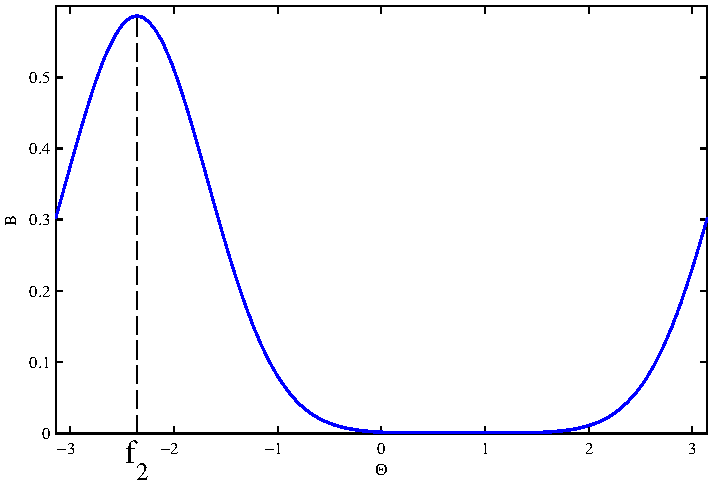
\includegraphics[width=\textwidth]{img/binExample.pdf}
	\end{subfigure}
\end{figure}
\end{frame}
%
\begin{frame}[c]{Descriptors}
\begin{itemize}
	\item GO
	\vspace{0.4cm}
	\item SI
	\vspace{0.4cm}
	\item GO+SI
	\vspace{0.4cm}
	\item SIFT (Lowe, 2004)
\end{itemize}
\end{frame}
%
\begin{frame}{Image correspondence results}
\begin{figure}
	\hspace{0.6cm}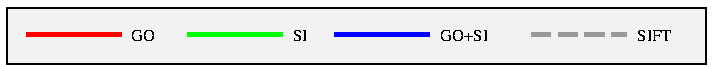
\includegraphics[width=0.9\textwidth]{img/dtuResults_opponent_legend_cropped.pdf} \\
	\begin{subfigure}[t]{0.49\textwidth}
		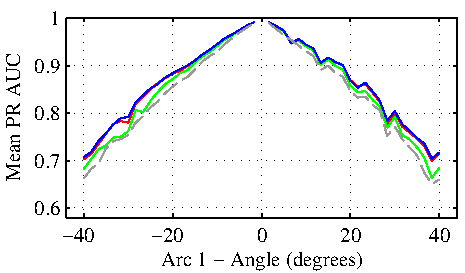
\includegraphics[width=\textwidth]{img/dtuResultsPR_opponent_1.pdf}
	\end{subfigure}
	\begin{subfigure}[t]{0.447\textwidth}
		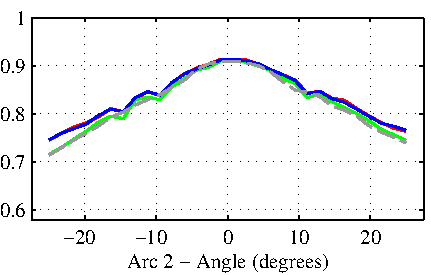
\includegraphics[width=\textwidth]{img/dtuResultsPR_opponent_2.pdf}
	\end{subfigure}
	\begin{subfigure}[t]{0.49\textwidth}
		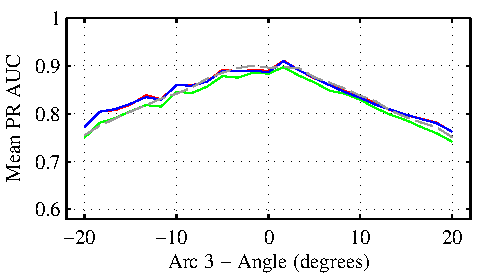
\includegraphics[width=\textwidth]{img/dtuResultsPR_opponent_3.pdf}
	\end{subfigure}
	\begin{subfigure}[t]{0.44\textwidth}
		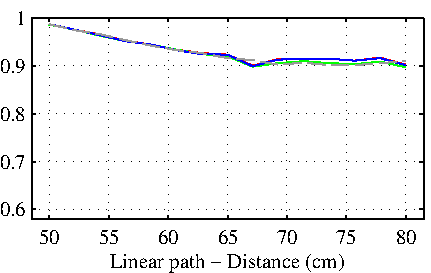
\includegraphics[width=\textwidth]{img/dtuResultsPR_opponent_4.pdf}
	\end{subfigure}
	\caption{Results on the DTU Robot 3D dataset}
\end{figure}
\end{frame}
%
\begin{frame}{Image correspondence results}
\begin{figure}
	\hspace{0.6cm}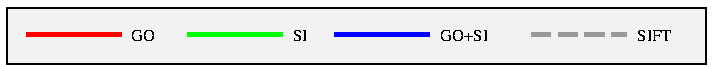
\includegraphics[width=0.9\textwidth]{img/dtuResults_opponent_legend_cropped.pdf} \\
	\begin{subfigure}[t]{0.5\textwidth}
		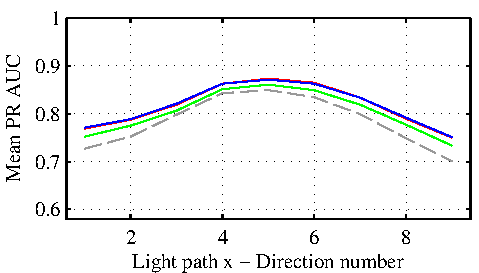
\includegraphics[width=\textwidth]{img/dtuResultsPR_opponent_5.pdf}
	\end{subfigure}
	\begin{subfigure}[t]{0.45\textwidth}
		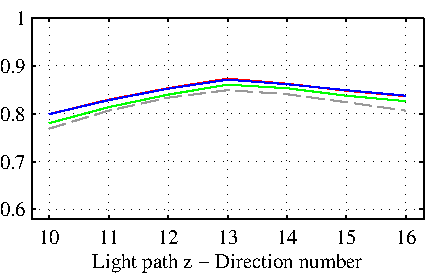
\includegraphics[width=\textwidth]{img/dtuResultsPR_opponent_6.pdf}
	\end{subfigure}
	\caption{Results on the DTU Robot 3D dataset}
\end{figure}
\end{frame}
%
\section{Pedestrian detection}
%
\begin{frame}{Sliding window}
\begin{figure}
\centering
%	\begin{subfigure}[t]{0.75\textwidth}
%	\end{subfigure}
	\animategraphics[width=0.9\textwidth,autoplay,loop]{2}{img/slidingWindow/position_}{001}{026}
\end{figure}
\end{frame}
%
\begin{frame}{Support vector machines}
\begin{itemize}
\item Binary classification of each window
\end{itemize}
\begin{figure}
	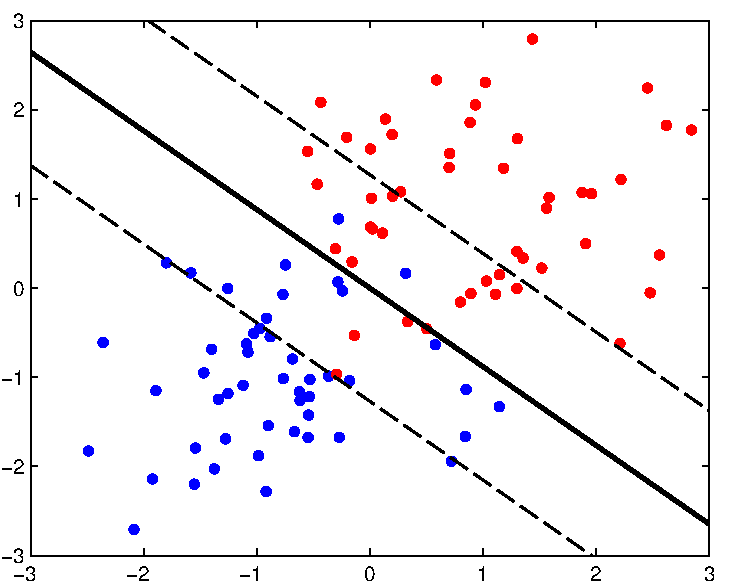
\includegraphics[width=0.75\textwidth]{img/svmExample.pdf}
\end{figure}
\end{frame}
%
\begin{frame}{Proposed descriptor}
\begin{minipage}[t]{0.49\textwidth}
\begin{itemize}
\item Uniform cell layout
\item No center aperture function
\end{itemize}
\end{minipage}
\begin{minipage}[t]{0.49\textwidth}
\begin{figure}
	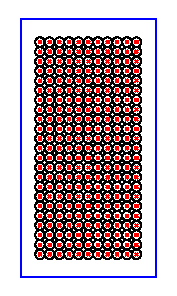
\includegraphics[height=0.7\textheight, clip=true, trim=9 9 9 9]{img/pedestrianWindowGrid.pdf}
\end{figure}
\end{minipage}
\end{frame}
%
\begin{frame}[c]{Descriptors}
\begin{itemize}
	\item GO
	\vspace{0.3cm}
	\item SI
	\vspace{0.3cm}
	\item GO+SI
	\vspace{0.3cm}
	\item Compact GO+SI
	\vspace{0.3cm}
	\item HOG (Felzenszwalb et al, 2010)
	\vspace{0.3cm}
	\item HOG+SI
\end{itemize}
\end{frame}
%
\begin{frame}{Pedestrian detection results}
\begin{figure}[tb]
\centering
	\hspace{0.54cm}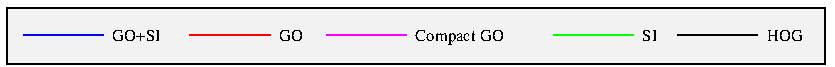
\includegraphics[width=0.935\textwidth]{../report/img/inriaTestResultsLegend.pdf} \\
	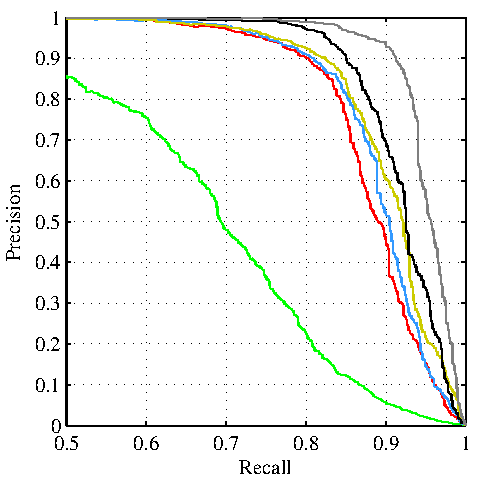
\includegraphics[width=\textwidth]{../report/img/inriaTestResultsPR.pdf}
	\caption{Results on the INRIA Person dataset}
	\label{fig:inriaTestResults}
\end{figure}
\end{frame}
%
\begin{frame}[c]{Project summary}
\begin{itemize}
	\item Studied the literature of descriptors
	\vspace{0.8cm}
	\item Developed a descriptor framework
	\vspace{0.8cm}
	\item Applied the framework to two problems
	\vspace{0.8cm}
	\item Extensive datasets used for evaluation
\end{itemize}
\end{frame}
%
\begin{frame}[c]{Conclusions}
\begin{itemize}
\item Image correspondence: Local normalization effective for light variations
\vspace{1cm}
\item Pedestrian detection: Shape index effective when used in combination with gradient orientations
\end{itemize}
\end{frame}
%
\begin{frame}[c]
\begin{center}
\begin{huge}
Thanks for listening!
\end{huge}
\end{center}
\end{frame}
%
\appendix
\begin{frame}{Additional slides}
\ghostframe
\end{frame}
\begin{frame}{Weight functions}
\ghostframe
\setlength{\jot}{15pt}
\begin{align*}
F_\text{norm}(\x) &= \frac{F(\x)}{\int F(\y) G(\y - \x; \eta \sigma_0) \,\text{d} \y} \\
A_j(\x) &= K(\x - (\x_0 + r \sigma_0 \c_j); \alpha k_j r \sigma_0) \\
P(\x) &= K(\x - \x_0; \rho r \sigma_0) \\
B(\x; f_i, f) &= K \left( f(\x) - f_i; \beta \frac{f_\text{max} - f_\text{min}}{2n} \right)
\end{align*}
\end{frame}
%
\begin{frame}{Kernels}
\ghostframe
\setlength{\jot}{15pt}
\begin{align*}
\mathit{Box} (x; \beta) &= 
\begin{cases}
    \frac{1}{2 \beta},& \text{if } |x| \leq \beta \\
    0,              & \text{otherwise}
\end{cases} \\
\mathit{Tri} (x; \beta) &= 
\begin{cases}
    \frac{1}{2 \beta} \left( 1 - \frac{| x |}{2 \beta} \right) ,& \text{if } |x| \leq 2 \beta \\
    0,              & \text{otherwise}
\end{cases} \\
G(x;\beta) &= \frac{1}{\sqrt{2\pi} \beta}
\exp\left( -\frac{x^2}{2 \beta^2} \right)
\end{align*}
\end{frame}
%
\begin{frame}{SIFT \cite{lowe2004distinctive}}
\ghostframe
\begin{minipage}[t]{0.7\textwidth}
	\begin{itemize}
	\item $4 \times 4$ square grid
	\item Trilinear interpolation
	\item Clipping of magnitudes
	\end{itemize}
\end{minipage}
\begin{minipage}[t]{0.25\textwidth}
	\begin{figure}
		
\includegraphics[width=\textwidth]{../report/img/siftGrid.pdf}
	\end{figure}
\end{minipage}
\end{frame}
%
\begin{frame}{HOG \cite{dalal2005histograms}}
\ghostframe
\begin{minipage}[t]{0.7\textwidth}
	\begin{itemize}
	\item $8 \times 16$ square grid
	\item Trilinear interpolation and clipping like SIFT
	\item Local normalization in $2 \times 2$ blocks
	\end{itemize}
\end{minipage}
\begin{minipage}[t]{0.25\textwidth}
	\begin{figure}
		
\includegraphics[width=\textwidth]{img/hogGrid.pdf}
	\end{figure}
\end{minipage}
\end{frame}
%
%[allowframebreaks]
\begin{frame}{References}
\ghostframe
\printbibliography
\end{frame}
%
\end{document}
